\documentclass[10pt,a4paper,twocolumn]{report}
%\documentclass[9pt,conference,compsocconf]{IEEEtran}

\usepackage{hyperref}
\usepackage{graphicx}	% For figure environment
\usepackage{verbatim}
\usepackage{xcolor}
\usepackage{amssymb}
\usepackage{amsthm}
\usepackage{mathtools}
\usepackage{biblatex}
\usepackage{multirow} % for combining rows
\usepackage{enumitem}
\usepackage{url}
\usepackage{amsfonts}
\bibliography{literature.bib}


\usepackage[justification=centering,
   format=plain]{caption} 
\graphicspath{{images/}}
\newcommand\todo[1]{\textcolor{red}{#1}}


\begin{document}
\title{Predictive Maintenance of Customer Premises Equipment using Machine Learning Techniques}



\author{
	
\includegraphics[width=0.2\linewidth]{EPFL}\\
	Hugo MOREAU\\
  	\begin{tt}hugo.moreau@epfl.ch\end{tt}, EPFL \\
	Data Science Laboratory (DLAB)\\
	Under the supervision of \\
	Pr. Robert West (Head of DLAB)\\
	Pratheep Ravy (Head of the Data Management Team)\\
	at UPC Schweiz GmbH during the Spring semester of 2018.
}

\maketitle{}
\setcounter{tocdepth}{4}
\tableofcontents
\abstract{
This paper summarises the method and findings of a Master Thesis conducted within the Data Management team of the broadband cable operator UPC Cablecom. The project aimed at building a proof of concept around the topic of router failure prediction. Every part of the process was discussed and the model was built from top to bottom. Many topics such has dataset construction, labeling propagation and model exploration are discussed extensively. This paper follows the empirical approach of research to justify iterative decisions. Among the five hundred thousand routers considered by the analysis 0.224\% were labeled as failing by this project. The final model considered, gradient boosted trees, allowed to predict the sickness of a router with a recall of approximately 14\% at 90\% precision level and 25\% at 80\% precision which supported the need for the company to move forward on such project and cultivate an internal competency around advanced data science. 
}

\chapter*{Introduction}
The increasing number of sensors and intelligence in most of our equipment has launched a new era. In order to kill the HIPPO\footnote{Highest Paid Person's Opinion}, our society is now heavily relying on data-driven decision. 

This shift was initiated by the spectacular increase in data collection. The amount of data to be analysed has become prohibitively high. That is the scenario at UPC Cablecom. The company has started to accumulate a lot of data: tracking the health of their equipment and most importantly of CPEs\footnote{Customer premises equipment (e.g. set top box, router, ...)}. 

The scope of this project is to leverage this data to improve customer experience. Combining customer feedback to CPE's health indicators, the final goal of the project is to build a Proof of Concept (POC) to determine whether data collected by the company could be used in order to increase the value that it captures (e.g. reducing the costs of servicing CPEs) or offered to their customer (e.g. increase customer satisfaction by proactively supporting them).

The project was articulated around five parts. We will start by giving an overview of the current situation of the company. This will allow us to follow with a thorough description of the way we were able to construct a dataset that would be usable to perform the desired analysis. This analysis was comprised most importantly of data preprocessing and exploratory analysis, an attempt to cluster the data and finally failure prediction. We will then discuss the performance of the classifier that we have built and of the different steps the project followed. Finally, we will briefly conclude on the project and its benefits for the firm. 

One could wonder why we decided to cluster the data. We will extensively discuss this point at a later stage but as an initial approach we could indicate that we couldn't trust our labelling because of the imperfections in the data collected so far.

As a final remark we would like to express our desire to make this report as thorough as possible given the different choices that have been made (but also the concessions) to make the work reproducible and also to give a sense of the scientific path that was followed.

\chapter{UPC Cablecom's Business}
In this chapter we will present the specificities of the company both in terms of network architecture, identified problems, data sources, and setup of the project.

\section{Hybrid Fiber-Coaxial Architecture}
\label{sec:HFC_archi}
Introduced in the 1990s, the Hybrid fiber-coaxial (HFC)\cite{wiki:hfc} architecture describes a broadband network that combines optical fiber and coaxial cable. While it isn't necessary to understand the entire network for this project, we will introduce  a high-level picture of the network as some notions will be required later on to explain some terms and justify choices. 

\vspace{2 \baselineskip}
The project uses measurements that are polled at different levels of the network to determine the "health" of a CPE. Therefore having a clear picture of the topology of the network will later prove to be useful. 

\begin{figure}[ht]
    \begin{center}
    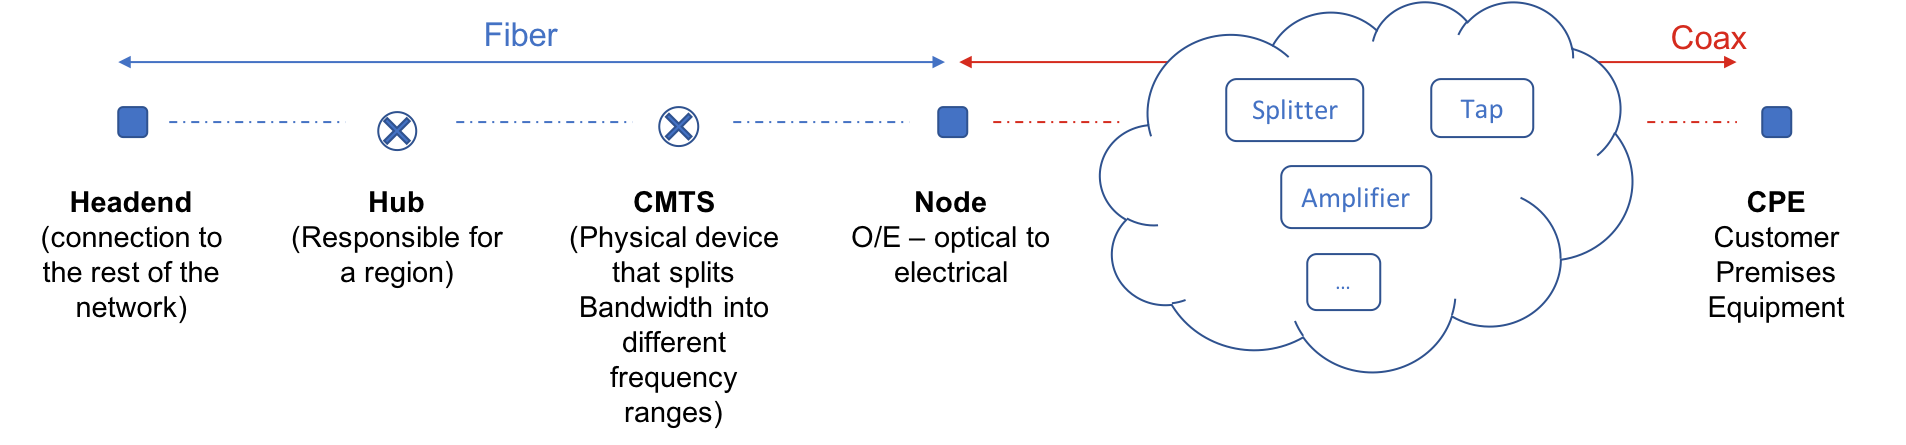
\includegraphics[width=1\linewidth]{HFC}
    \end{center}
    \caption{Hybrid Fiber-Coaxial Topology of the Network}
    \label{HFC}
\end{figure}

Figure~\ref{HFC} illustrates this topology and more specifically how a CPE is connected to the rest of the network. Among nodes that compose the network only two are considered as active and are regularly polled to monitor their behaviour: CPE and CMTS\footnote{Cable Modem Termination System}.

\begin{figure}[ht]
    \begin{center}
    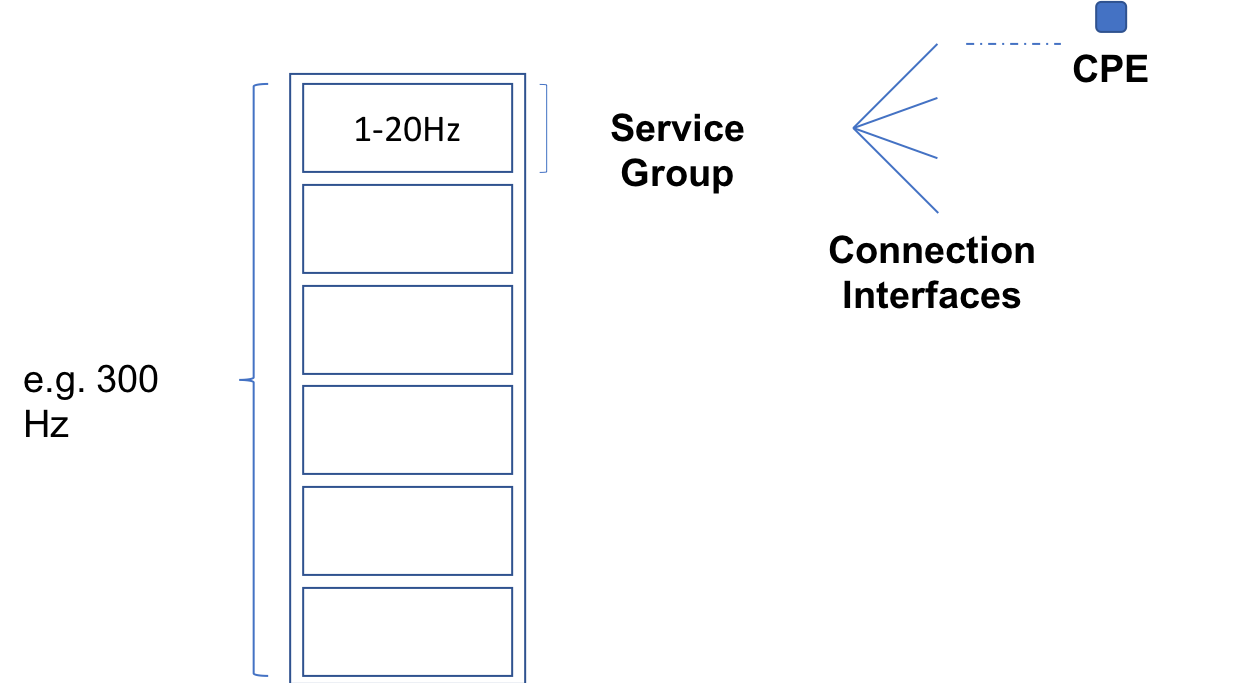
\includegraphics[width=0.5\linewidth]{SVG}
    \end{center}
    \caption{Details of the CMTS decomposition}
    \label{SVG}
\end{figure}

A CMTS splits the bandwidth it receives into multiple frequency ranges that are called Service Groups. A Service Group itself contains multiple connection interfaces as it can be observed in Figure~\ref{SVG}. Each CPE connects to a connection interface. The interface that is chosen depends on many parameters (e.g. load of the interface) and changes frequently. 

On the other hand, the association between a CPE and a service group does change as well but at a much slower rate (by order of days). 

\section{Problem Identified}
As opposed to some other providers, UPC owns the network it uses. Therefore the company has the opportunity to challenge the status quo. It has been polling regularly nodes of the network to perform passive operations. That gives it a myriad of possibilities to use all the data that is being collected but also future perspective of enriching it in order to build new tools and solutions.

As of today, the brand has trouble to understand customer behaviours. Because it cannot detect all problems if customers do not express any complaint, it cannot track how customers react to particular problems. As an example Teia Fetescu, a manager in THD\footnote{Technical help desk} Processes and Support Improvement, has expressed her frustration regarding how sometimes they witness a lot of complaints on social media about a particular problem but never received any calls regarding such problem and hence couldn't identify the symptoms and solve the problem. 

Therefore, we believe that we could leverage the data that UPC is using in order to identify CPEs that are failing and be able to do something about it. By having the capability to detect such problems the company could: go from passive to proactive troubleshooting, analyse how their customer reacts to given problems, and diagnose faster recurring problems.

\section{Data Sources}
As mentioned earlier, UPC collects a lot of data from its network in order to be able to troubleshoot problems, monitor its state, etc. We won't discuss all the data sources that have been used to fetch some minor information used along this project but rather give the two initial and main sources that were identified to be potentially leveraged by machine learning algorithms. As we should explain it in Section~\ref{sec:setup}, we will use data that is already being collected by UPC for different business needs:

\begin{itemize}
	\item ServAssure (SAA): Every 15 minutes, CMTS interfaces and CPEs are polled. Multiple measurements are monitored by such polling (e.g. Sound to Noise ratio, transmission power,...). Given the large number of such items it is impossible for UPC to keep a complete history of such polls. It aggregates them hourly and stores them for 11 days (10 full past days in addition to the current day). We would like to use this source in order to extract significant indicators of a CPE's Health.
	\item Virtual Interactive Assistant (VIA): interactions with the THD are tracked by the company in order to perform some reporting and also to be able to see a customer's history. This source is not very reliable as it depends on human interaction (the THD agent that answers the phone) with the software that helps them diagnose customers' problems. We were convinced that a proper filtering applied to this data would help us flag failing CPEs. It is important to note, though, that this isn't exactly flagging all the failing CPEs (e.g. some customers may not call the customer center when experiencing some problem).
\end{itemize}

\section{Setup of the Project}
\label{sec:setup}
First of all, it is important to note that this project was to the eyes of UPC a simple Proof of Concept that would help them determine the value that resides in the data that they own. This means that the support and resources available for conducting the project were fairly limited. 

As it is mentioned in the title, it was conducted inside the Data Management team. Members of the team have very limited knowledge concerning Data Analysis and Machine Learning. Nevertheless, because of their frequent interaction with the different data sources they had an overview of what data was available and how we could use it in order to build an innovative tool to answer business needs. Because of this framework, we had to reach out to different people in order to get help regarding the multiple components of this project:
\begin{itemize}
	\item Jonas Staempfli (\texttt{Jonas.Staempfli@upc.ch}): HFC support expert. Helped on understanding the network measurements and the way to use them in order to decide on the potential "failures" of CPEs.
	\item Felix Reisen (\texttt{Felix.Reisen@upc.ch}): Advanced Analytics inside the Business Intelligence team. Helped at supervising the different parts of the project from feasibility to implementation.
\end{itemize}

The project was realised during a heavy workload period and support proved to be a scarce resource. This is one of the points we will discuss before the conclusion, the knowledge regarding UPC’s business was complicated to obtain as it was detained by many different actors that may not have the time to deliver such piece of information. 

Finally, the POC was to use only the data that was already available as we couldn't afford (in terms of time nor budget) to organise the collection of new measurements on the CPE that could have been more helpful to diagnose.

\vspace{1\baselineskip}
The different terms are now introduced as well as the technical framework of the project. This should give the reader an understanding of the potential and challenges of this project. The final aim of the project should be clear ahead of this thesis as it will justify many choices and drive the research.


\chapter{Dataset Construction}
As opposed to datasets that are widely used in Machine Learning classes at university, in the professional world those are much less frequently available and need to be built on the spot for specific tasks. The major challenge of this project was the data collection part. We needed to determine what was available, what we should use, how to collect it, aggregate it and represent it. 

This protocol was the result of an iterative process of interviews with different stakeholders. Often we had to avoid a given source because initial analysis revealed that the data wasn't usable. The lack of strong documentation of the content of databases certainly made this process longer than expected.

In this chapter we will discuss first how we managed to identify failing \acrshort{cpe}s, we will give an overview of the different measurements that we used to characterise a given \acrshort{cpe}'s health. We will then look at the representation of such measurements to encompass both the notion of time but also to get rid of unwanted idiosyncrasies in the data. We will follow on presenting choices that were made to restrict the dataset and avoid particular cases that lied outside of the scope. Finally, will be presented the strategy that was derived in order to automatise data collection in the most resilient and efficient way.

\section{Identifying Un-heatlhy \acrshort{cpe}}
\subsection{Understanding \acrshort{via}}
Before we get started, it would be useful to define the different keywords that are proper to the way \acrshort{via} stores data. 

When a customer requires technical support, the employee will use \acrshort{via} to service the customer's problems. This software will perform some live measurements to help the employee in the support process. The database is filled by the software but based on the interaction with the agent. 

Whenever a customer calls, a \textbf{session} is started. Each session is composed of multiple \textbf{events} that are launched while the agent interacts with the customer. During a session the agent may start multiple flows. A \textbf{flow} corresponds to the process that the agent follows to diagnose and solve a particular problem that the customer is experiencing. Because he might not know at first which flow is the most appropriate, he will most often start many flows and try to find out which one solves the problem. During a flow execution, the software will emit \textbf{milestones} in order to keep track of the execution of the flow, one for each event. 

Also a \textbf{case} will be created for one or more sessions\footnote{This seems, according to the reporting team, to be a Data Quality issue as first it was intended to be a one to one relationship. But in our scenario we only care to have a unique case for a given session to get the details.} in order to log in an interaction between the customer and the service center. It will give us information regarding the customer details (e.g. the account number that will allow us to recover the Medium Access Control addresses (\acrshort{mac}) of devices that belong to the customer).

\subsection{Protocol to Flag Failing \acrshort{mac}s}
\subsubsection{Labeling Sessions With a Problem}
Our initial goal was to be able to label the problem that is being solved in a given session. Milestones are human readable description of the specific steps of a particular flow, therefore they would be a perfect way for us to attribute a string to a given problem. The challenge was the many events and therefore milestones that are emitted during a particular flow. But also, the many flows that can coexist in a session as explained earlier.

We started by focusing the research on full flows: these are flows that have been completed successfully and yielded the end of the call. In order to detect such flows, we used two flags that are present for each milestone : \texttt{CNT\_INTERACT\_SENT} and \texttt{CNT\_CASE\_SENT}. Whenever one of these two flags (found in table \texttt{SCO.REP\_VIA\_MILESTONE\_V}) is positive then it means that we have found a milestone in a flow that finished the interaction between the agent and the customer. With such strategy we could flag "full" flows.

Then we needed a strategy to choose which milestone to use inside a full flow. This was decided arbitrarily and thanks to the advice of the reporting team. The very first milestone of a full flow would be general enough to give us a problem label. As events inside a session are sequential (not depending on what flow emitted them), we had to look for the minimum event number that had the same flow identifier as the flow determined as "full" in the session. 

\subsubsection{Linking Sessions to Devices}
Another challenge was that we do not store anywhere what is the \acrshort{cpe} that is experiencing problems in the case of the identified sessions. Moreover, it can happen that the customer has multiple \acrshort{cpe}s at home (e.g. one of the boxes commercialised by UPC had trouble to cover a full apartment with Wi-Fi and therefore the company started offering a two-room solution with two Internet-capable devices). 

Because we couldn't find any way to link a particular device to a session we decided to flag all the \acrshort{mac}s of a customer as failing whenever we found a session concerning this particular user. In order to determine what user corresponds to each session we had to join tables \texttt{SCO.REP\_VIA\_CASE\_V} and \texttt{SCO.REP\_VIA\_SESSION\_V} based on \texttt{ID} and \texttt{JOURNAL\_ID} respectively. 

Finally, another problem arose: \acrshort{cpe}s do not necessarily have only one \acrshort{mac}, this is due to the fact that they may use multiple connection interfaces to provide different services (e.g. the Horizon Box provides phone, digital TV and Internet using the network). A first attempt was made to use what is called \textbf{the management \acrshort{mac}} which should be the one that is used in \acrshort{saa} to identify polled \acrshort{cpe}. It yielded poor results (almost no match between management \acrshort{mac}s and those in \acrshort{saa}). Therefore we used another table that was being developed \texttt{DM\_TOPO\_CH.ETL\_STG\_NW\_TOPO\_NODES}. It aims at providing topology information of the network and surprisingly the \acrshort{mac}s extracted from this table yielded much more matches with \acrshort{saa}. The only filtering we had to perform was to focus on nodes with \texttt{topo\_node\_type\_id = 55} as it references \acrshort{cpe} nodes. 

\subsubsection{Ensuring the Exactitude of Our Labeling}
Once we had all these \acrshort{mac}s labeled with a particular problem, we were made aware that a specific session even though it contained a full flow may not have solved the problem of the customer (to be opposed to what is called a \acrfull{ftr}). In order to increase our confidence that the label we gave to the problem  was correct, we had to use yet a different data source \texttt{SCO.REP\_CLY\_INTERACTION\_V}. This table constructed for reporting purposes has a flag called \texttt{FLG\_FTR\_7D\_FLG}. It attempts to check whether the customer called \acrshort{thd} in the following 7 days for the same kind of problem\footnote{The exact logic behind the flag was not available to us but the Business Intelligence team testified that we could trust it as they had already used it in some analysis which offered good results.}. 

This reporting table is built on top of \acrfull{cly}, a service which deals with a more general type of interaction. The challenge was that there is no one-to-one mapping between \acrshort{cly} interactions and \acrshort{via} interactions. We decided that given that the \acrshort{ftr} flag was anyway an estimate we could perform a fuzzy matching between the two. This would still allow us to increase our confidence in the labeling. The assumptions that were formulated were:
\begin{itemize}[topsep=0pt,noitemsep]
	\item The \acrshort{via} case and \acrshort{cly} interaction started on the same day
	\item As \acrshort{via} logs a \acrshort{cly} interaction the timestamp of \acrshort{via} should not be prior to \acrshort{cly} one
	\item Account numbers (the customer) of both match
	\item Employee IDs match as well
\end{itemize}
It happened that this would yield multiple matches and we decided to always take the match from clarify which creation timestamp is the closest to the one in \acrshort{via} as this was the only strategy that we could follow (even checking by hand we couldn't determine the correct match as we had already used all fields that are common between the two sources). 

\subsubsection{Focusing on Certain Problems}
In accordance with the \acrshort{hfc} support expert, we decided to limit our analysis to Internet Problems (which we could do by focusing on Internet Flows in \acrshort{via}) as those would probably be the one to be the most easily identifiable from the \acrshort{saa} data. But also because it would allow us to restrict the analysis to particular \acrshort{cpe}s that have Internet capabilities. 

We realise that this is an arbitrary choice and will discuss later that we may be discarding a lot of detectable problems in the analysis. Nevertheless it also allowed us to focus the research on particular use cases and was validated both with the thesis supervisor (from whom the idea came from originally) and Felix Reisen. 

\section{Characterising \acrshort{cpe}s}
\subsection{Measurement Choices}
\label{subsec:mes_choices}
Choosing the correct measurements to monitor the health of \acrshort{cpe}s required the help of Jonas Staempfli as he had the knowledge regarding how such measurements evolve over time, what normal and abnormal values are, what the time granularity that should be considered to detect problems is and many other tasks specific information. 

As stated earlier, we have at our disposal two types of active nodes in the network that are polled: \acrshort{cpe} and \acrshort{cmts} interface. 

\subsubsection{Available Values}
We started by presenting to the expert all the measurements that we had at hand and asked him to help us choose those that would be the most promising for our prediction task. We have first discussed the measurements available at the \acrshort{cpe} level that were found in \texttt{SAA.CM\_HOUR\_HEALTH}, and we describe in Table~\ref{CPEMes} the features that we decided to keep.

\begin{table}[h]
\begin{center}
\begin{tabular}{c l}
\hline
\textbf{Feature} & \textbf{Description}\\ 
\hline\hline
\texttt{TXPOWER\_UP} & The average upstream transmitting power.\\
\hline
\texttt{RXPOWER\_UP} & The average upstream receiving power.\\
\hline
\texttt{RXPOWER\_DN} & The average downstream receiving power.\\
\hline
\texttt{CER\_DN} & Maximum codeword errors downstream.\\
\hline
\texttt{CER\_UP} & Maximum codeword errors upstream.\\
\hline
\texttt{SNR\_DN} & Sound to noise ratio downstream.\\
\hline
\texttt{PCT\_TRAFFIC\_DMH\_UP} & Percentage of upstream traffic computed as degraded modem hours.\\
\hline
\texttt{PCT\_TRAFFIC\_SDMH\_UP} & Percentage of upstream traffic computed as severally degraded modem hours.
\end{tabular}
\end{center}
\caption{\label{CPEMes}Features at the \acrshort{cpe} level}
\end{table}

Regarding \acrshort{cmts} interfaces we decided to monitor certain measurements because they could give us indications about the group of \acrshort{cpe}s we are looking at. A previous project called Common Path Distortion showed that frequently when a particular node is experiencing problems in a group of nodes then it may affect the whole group. Therefore we repeated the analysis with Jonas regarding which measurements extracted from \texttt{SAA.CMTS\_HOURS\_UPSTREAM\_STATS} (for the upstream channel) and \texttt{SAA.CMTS\_HOURS\_DNSTREAM\_STATS} (respectively for downstream) would serve our purpose. Features that we retained are grouped in Table~\ref{CMTSMes}.

\begin{table}[h]
\begin{center}
\begin{tabular}{c l}
\hline
\textbf{Feature} & \textbf{Description}\\ 
\hline\hline
\texttt{UTILIZATION\_UP} & Maximum percent utilization of upstream.\\
\hline
\texttt{RXPOWER\_UP} & Average power being received by \acrshort{cmts} on interface (upstream).\\
\hline
\texttt{TXPOWER\_UP} & Average power transmitted from CMs on interface (upstream).\\
\hline
\texttt{CER\_UP} & Maximum Codeword Error Ratio for interface (upstream).\\
\hline
\texttt{MS\_UTILIZATION\_UP} & Percent minislot utilization of upstream (upstream).\\
\hline
\hline
\texttt{UTILIZATION\_DN} & Maximum percent utilisation of downstream.\\
\hline
\texttt{RXPOWER\_DN} & Average power being sent by \acrshort{cmts} on interface (downstream).\\
\hline
\texttt{CCER\_DN} & Maximum Corrected Codeword Error Ratio for interface (downstream).\\
\hline
\texttt{CER\_DN} & Maximum Codeword Error Ratio for interface (downstream).\\
\hline
\texttt{AVG\_SNR\_DN} & Average carrier to noise ratio for interface (downstream).\\
\end{tabular}
\end{center}
\caption{\label{CMTSMes}Features at the \acrshort{cmts} interface level}
\end{table}

For each active node all of these measurements are available at a one-hour granularity for 10 full days and we shall discuss in Section~\ref{subsubsec:time_representation} how we used such measurements.

Also we have decided to add, what we referred to as, \textbf{static information}, because they are not time dependent (or at a much greater time granularity with e.g. \texttt{N\_CPE\_BUILDING} presented in Section~\ref{subsubsec:constructed_features}. It will not drastically change over periods that are less than a week except in very particular cases that we considered as minor). These pieces of information are used to either identify the \acrshort{cpe} or track some relevant metrics and are explained in Table~\ref{StaticInfos}.

\begin{table}[h]
\begin{center}
\begin{tabular}{c p{100mm}}
\hline
\textbf{Feature} & \textbf{Description}\\ 
\hline\hline
\texttt{DAY\_0} & As we will explain in Section~\ref{subsubsec:time_representation}, we will aggregate the data at different periods. Therefore each measurements' vector will be relative to a given Day\textsubscript{0}.\\
\hline
\texttt{\acrshort{mac}} & Unique identifier of the \acrshort{cpe}.\\
\hline
\texttt{CLY\_ACCOUNT\_NUMBER} & Unique identifier of the customer in \acrlong{cly}.\\
\hline
\texttt{SAA\_ACCOUNT\_NUMBER} & Unique identifier of the customer in \acrlong{saa} (under Pratheep's advice we decided to keep both account numbers as they could sometimes differ. So far we have yet to find such a case, but it would help us make sure we know how to link the failing \acrshort{cpe} back to a customer).\\
\hline
\texttt{HARDWARE\_MODEL} & Either to facilitate later analysis of the distribution of problems among \acrshort{cpe}s  or to be able to take into consideration what type of hardware we are diagnosing during classification (we suppose that this could influence the values of different features).\\
\end{tabular}
\end{center}
\caption{\label{StaticInfos}Static information collected for each \acrshort{cpe}}
\end{table}

\subsubsection{Constructed Features}
\label{subsubsec:constructed_features}
Aside from these measurements that we arbitrarily selected with the help of the expert, we decided to explore what other measurements could be added in order to characterise as well as possible \acrshort{cpe}s' health. The measurements that we have derived can be found in Table~\ref{CreatedMes}.

\begin{table}[h]
\begin{center}
\begin{tabular}{c p{100mm}}
\hline
\textbf{Feature} & \textbf{Description}\\ 
\hline\hline
\texttt{OFFLINE} & A good indicator of a \acrshort{cpe} experiencing problem could be its status on the network (being online or offline). This information could be derived from \texttt{SAA.CM\_HOUR\_HEALTH} where a \texttt{CM\_STATUS != 8} indicated an offline \acrshort{cpe}.\\
\hline
\texttt{MISS\_*} & Missing values are usually hidden when doing machine learning using imputation, that is we will replace them using some arbitrary values (e.g. mean of the feature, 0, ...). In our case these missing values are missing not at random (MNAR \cite{wiki:mnar}). Later we aggregate these values at the database level and might lose the information about what was missing. So we added \texttt{MISS\_*} that will give for each aggregate (c.f. Section \ref{subsubsec:time_representation}) the percentage of aggregated values that were missing.\\
\hline
\texttt{N\_CPE\_BUILDING} & A given building will have the same signal carrier for all \acrshort{cpe}s. According to the \acrshort{hfc} expert, it could make sense to look at the number of \acrshort{cpe}s that are inside the same building in order to take it into consideration when classifying. Again this information was found in the \texttt{M\_TOPO\_CH.ETL\_STG\_NW\_TOPO\_NODES} table (\textit{Note that this feature is also static}).\\
\end{tabular}
\end{center}
\caption{\label{CreatedMes}Features constructed to enrich existing measurements}
\end{table}


\subsection{Representation Choices}
Now that we have discussed what features could be used for our prediction task, we would like to present the different choices that have been made to properly represent the data. We had to derive different strategies. 

\subsubsection{Linking \acrshort{cmts} Interfaces to \acrshort{cpe}}
We explained in Section~\ref{sec:HFC_archi} that it is somehow challenging to link a \acrshort{cmts} interface to a \acrshort{cpe} as it can change dynamically and very frequently. Therefore we had to design with Jonas Staempfli a workaround to be able to link the \acrshort{cmts} interface measurements presented in Table~\ref{CMTSMes} with \acrshort{cpe} measurements presented in table~\ref{CPEMes}. The most coherent grouping we found was to use the service group as a logical grouping of \acrshort{cpe}s. 

Therefore the \acrshort{cmts} interfaces measurement were averaged over all the interfaces of a given service group and presented as the measurements at the service group level. We found the mapping between interfaces in table \texttt{DM\_DIM.ETL\_STG\_TOPO\_CMTS2NODE}.

\subsubsection{Decreasing Group Specificities}
Then we wanted to make sure that we could work with relative data. While discussing with different stakeholders at UPC, we discovered that it was very common to have a group of \acrshort{cpe}s with abnormally high values for certain measurements even though they were not experiencing any issues.

This drove us to scale the \acrshort{cpe} features in each logical group (the Service Group) in order to get rid of these specificities and hopefully obtain relative values that would be comparable between \acrshort{cpe}s in different locations of the network tree. 

\subsubsection{Including the Time Dimension of Failures}
\label{subsubsec:time_representation}
We cannot detect failure at the exact time they happen. This is why we need to collect data over an extended period of time for each \acrshort{cpe} failure such that we give our classifier the history of the \acrshort{cpe}s' behavior to let it flag the outlying values. 

Discussing with the \acrshort{hfc} support expert, he first advised us not to consider a time granularity that would be too fine. Indeed health measurements of \acrshort{cpe}s can 'flap' without any real connection to a potential problem (e.g. due to electromagnetic fields or change in temperatures). 

Also as we already have a large number of values it would make sense not to keep all time measurements but rather to aggregate these measurements over different time granularities:
\begin{itemize}
	\item Last 24 hours: this was what we estimated as the most probable time when failure happened (usually customers would not wait that long in case of service degradations before reaching out). Over the last 24 hours we considered 6 hour windows on which we averaged all measurements.
	\item Last 6 days: this was considered as the maximum amount of time a customer could wait before calling \acrshort{thd}. For this period we took a longer averaging window of 1 day to limit the resulting number of features (this is a tradeoff that will be discussed in final parts).
\end{itemize}

Then we also found out that what we are really interested in isn't the absolute value of a measurement but rather its evolution over time. Therefore we decided to present a given time aggregate as a difference between the current aggregate and the previous one in order to only display the evolution of these aggregates over time. 

Therefore if we consider a measurement $x$ and denote by $x^d_i$ for $i \in \{0,..23\}$ and $d \in \{0,...,-5\}$  the polled version of x at the $i^\text{th}$ hour of day $d$ (where d is relative to Day\textsubscript{0}). We will construct : 

\begin{equation}
\begin{cases}
	\hat{x}_{6h} &= (x^0_{23}+...+x^0_{18})/6 - (x^0_{17}+...+x^0_{12})/6\\
	\hat{x}_{12h} &= (x^0_{17}+...+x^0_{12})/6 - (x^0_{11}+...+x^0_{6})/6\\
	\hat{x}_{18h} &= (x^0_{11}+...+x^0_{6})/6 - (x^0_{5}+...+x^0_{0})/6\\
\end{cases}
\end{equation}

This means for example that $\hat{x}_{18h}$ is the average of the 6 hour window that started 18h before midnight on Day\textsubscript{0} represented as the difference with respect to the previous window. To ease up comprehension, we present the operation on Figure~\ref{6h_agg}.

\begin{figure}[ht]
    \begin{center}
    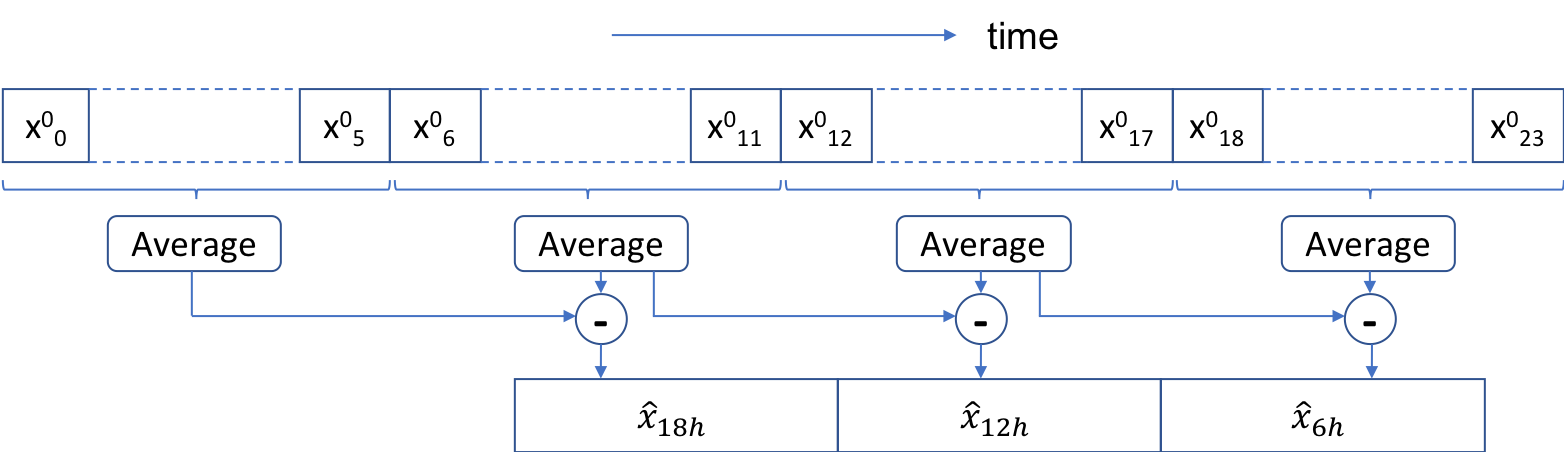
\includegraphics[width=1\linewidth]{6h_aggregation}
    \end{center}
    \caption{The aggregation over the last 24 hours with 6 hour window averaging and relativisation of averages with respect to the past aggregate}
    \label{6h_agg}
\end{figure}


And then we construct:

\begin{equation}
\begin{cases}
	\hat{x} &= (x^0_{23}+...+x^0_{0})/24\\
	\hat{x}_{1d} &= (x^0_{23}+...+x^0_{0})/24 - (x^1_{23}+...+x^1_{0})/24\\
	...\\
	\hat{x}_{5d} &= (x^4_{23}+...+x^4_{0})/24 - (x^5_{23}+...+x^5_{0})/24\\
\end{cases}
\end{equation}

The principle is identical to what we do with 6 hour averages.

By allowing these two granularities we have constructed a vector that gives us the history of values over multiple days and hours. It is important to note that not all measurements were represented as relative differences w.r.t. their previous average. Regarding \texttt{OFFLINE} and \texttt{MISS\_*} it would not make sense to make such relative\footnote{Because their magnitude actually matter more than their evolution on the long run.}, so we simply represented them as their averages (therefore for the last 24 hours they are represented as 4 values e.g. \texttt{OFFLINE\_PCT\_6H}, \texttt{OFFLINE\_PCT\_12H}, \texttt{OFFLINE\_PCT\_18H}, \texttt{OFFLINE\_PCT\_24H} which are simply the averages from the first up to the 4th furthest 6h window).

\section{Restricting the Dataset: Offline \acrshort{cpe}s}
\subsubsection{Outliers Detection}
During our initial analysis we realised that offline \acrshort{cpe}s wouldn't have any polled values and that would be a problem. With rising ecological concerns and energetic awareness, it seems like many people turn off their electronic at night. We didn't have any simple way to verify this gut feeling so we decided to prevent it by filtering our dataset. Nevertheless we couldn't take out all offline \acrshort{cpe}s as this could be already eliminating outliers that are indeed failing \acrshort{cpe}s. 

We had 10 days of data in \acrshort{saa} that we could use in order to detect these outliers. Using the \texttt{OFFLINE} feature that we constructed for each measurement, we could compute for each \texttt{HARDWARE\_MODEL} what would be standard offline times. In order to find such standard offline time we looked at the 99\textsuperscript{th} percentile (the value that will separate the population into a 99\% that we keep and 1\% we discard) of the offline frequency at a given hour of the day computed over all the days of history. To put things simply with 10 days of data, we look at the measurements made at 3am. Our assumption is that if someone turns off their \acrshort{cpe} during the night then he will have a frequency of being offline at 3am of $100\%$ which will be detected with respect to a \acrshort{cpe} that has an issue once in a while at 3am causing it to be offline. We took out any \acrshort{cpe} that was an outlier for any given hour. 

We made it relative to a particular model as some models may be more prone to errors causing them to be more offline than others, the underlying desire was to compare only pieces of hardware that are comparable. 

\subsubsection{Accidental Discovery: Automatic Deep Sleep Mode}
While performing this analysis we observed surprising results. We plotted for each type of hardware model the cutoff values that were obtained. Because the 99\textsuperscript{th} percentile was a bit too discriminative to see much, we looked at the 80\textsuperscript{th}. As it can be observed on Figure~\ref{offline}, the cutoff values for Media Box and Horizon Box are alarmingly high. It means that for such devices most of the population is offline during most of the day. 

\begin{figure}[ht]
    \begin{center}
    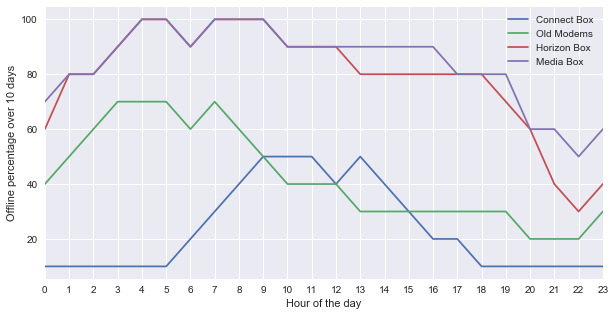
\includegraphics[width=1\linewidth]{offline}
    \end{center}
    \caption{80\textsuperscript{th} centile per hour of the day by Hardware type in terms of offline percentage computed over 10 days of history}
    \label{offline}
\end{figure}

By presenting these results to different stakeholders and mostly the \acrshort{hfc} support team we discovered that we had forgotten about a particular feature of most recent \acrshort{cpe}s: automatic deep sleep mode. UPC is obligated by law on all new models to automatically turn off the \acrshort{cpe} if it hasn't been used for a given period of time. Also this feature is enabled by default and hence will affect most of the models that have it built in. These models had to be taken out of our analysis as they would present a lot of missing measurements and possibly give false training patterns to our model.

\begin{table}[h]
\begin{center}
\begin{tabular}{c l r r}
\hline
\textbf{Type} & \textbf{\texttt{Hardware Model}} & \textbf{Offline \%} & \textbf{\acrshort{saa} \%}\\ 
\hline\hline
\multirow{3}{*}{Horizon Box} 		& \textbf{HORIZON HD RECORDER}					& $27.23\%$ 			& $\mathbf{18.80\%}$\\
									& \textbf{HORIZON HD RECORDER (G7401)} 			& $20.95\%$ 			& $\mathbf{15.07\%}$\\
									& HORIZON VSC									& $0\%$ 				& $0\%$\\
\hline						
Connect Box							& \textbf{CONNECT BOX CH7465LG COMPAL}			& $23.42\%$ 			& $\mathbf{41.16\%}$\\
\hline
\multirow{6}{*}{Mediabox} 			& MEDIABOX RECEIVER THOMSON DC152UPC 			& $0.04\%$ 				& $0.02\%$\\
									& MEDIABOX HD PHILIPS DCR8111/03 				& $0.01\%$ 				& $0\%$\\
									& MEDIABOX RECORDER HD CISCO						& $1.43\%$ 				& $0.74\%$\\
									& MEDIABOX RECORDER HD CISCO 8685				& $4.70\%$ 				& $3.05\%$\\
									& \textbf{MEDIABOX HD PACE DCR7111}				& $12.83\%$ 			& $\mathbf{7.02\%}$\\
									& MEDIABOX HD PHILIPS DCR7101/03					& $0.04\%$ 				& $0.02\%$\\
\hline
\multirow{6}{*}{Old Modems} 			& UBEE EVM3236 (ED 3.0) - CPE 					& $2.13\%$ 				& $2.94\%$\\
									& UBEE EVM3206 (ED 3.0) - CPE 					& $1.46\%$ 				& $1.72\%$\\
									& WLAN MODEM TC7200 - CPE						& $2.79\%$ 				& $4.62\%$\\
									& WLAN MODEM EVW3226 - CPE						& $0.56\%$ 				& $0.86\%$\\
									& WLAN MODEM TC7200 V2 - CPE						& $1.05\%$ 				& $1.89\%$\\
									& WLAN MODEM TWG870 - CPE						& $1.23\%$ 				& $1.92\%$\\
\hline 
\multirow{13}{*}{FTTH (Left out)} 	& FTTH\_CPE\_UBEE EVM3206 (ED 3.0) - CPE 		& $0\%$ 				& $0\%$\\
									& FTTH\_CPE\_UBEE EVM3236 (ED 3.0) - CPE 		& $0\%$ 				& $0\%$\\
									& FTTH\_CPE\_CONNECT BOX CH7465LG COMPAL			& $0.04\%$ 				& $0.08\%$\\
									& FTTH\_CPE\_HORIZON HD RECORDER					& $0.03\%$ 				& $0.02\%$\\
									& FTTH\_CPE\_HORIZON HD RECORDER (G7401)			& $0.04\%$ 				& $0.03\%$\\
									& FTTH\_CPE\_MEDIABOX HD PACE DCR7111			& $0.01\%$ 				& $0.01\%$\\
									& FTTH\_CPE\_MEDIABOX RECORDER HD CISCO 8685	& $0.01\%$ 				& $0\%$\\
									& FTTH\_CPE\_WLAN MODEM TC7200 V2 - CPE			& $0\%$ 				& $0\%$\\
									& FTTH\_CPE\_WLAN MODEM TC7200 - CPE				& $0\%$ 				& $0\%$\\
									& FTTH\_CPE\_WLAN MODEM TWG870 - CPE				& $0\%$ 				& $0\%$\\
									& FTTH\_CPE\_MEDIABOX HD PHILIPS DCR7101/03		& $0\%$ 				& $0\%$\\
									& FTTH\_CPE\_WLAN MODEM EVW3226 - CPE			& $0\%$ 				& $0\%$\\
									& FTTH\_CPE\_MEDIABOX RECORDER HD CISCO			& $0\%$ 				& $0\%$\\

\end{tabular}
\end{center}
\caption{\label{CPEProportions}Internet Capable \acrshort{cpe}s, their proportion among \acrshort{saa} measurements, and the proportion among all measurements from such \acrshort{cpe}s marking the \acrshort{cpe} as offline. (Note that percentages have been rounded.)}
\end{table}

In the table~\ref{CPEProportions}, we have described all Internet-capable \acrshort{cpe}s and highlighted those that have the highest frequency in the dataset. According to Business Intelligence, the FTTH \acrshort{cpe} can be left out of the analysis as they do not correspond to hardware used by customers. Horizon Box and Media Box must be left out of the analysis as stated above due to their deep sleep mode. Therefore the only \acrshort{cpe}s that we considered in the analysis were the Connect Box and Old modems.

\section{Collecting the Data}
The restrictions on the type of \acrshort{cpe} analysed combined with the way we identify failing \acrshort{cpe}s yielded approximately $500,000$ \acrshort{mac}s considered every day and an average of $112$ daily failing \acrshort{cpe}s (representing $0.224\%$ of this analysed population).

So far we discussed the construction of vectors composed of five days of history. We will see in the following section that practically this construction was implemented in a different way for optimisation reasons. We shall also discuss the different techniques that have been used to make this data collection reproducible and automatised. 

\subsection{Collecting Over Multiple Days}
\label{subsec:collecting}
As stated earlier, \acrshort{saa} only keeps 10 days of history. Therefore we could not build a representative dataset from these 10 days of history (one of our concerns being that we would like to balance the dataset to improve training). Therefore we had to collect over multiple days to iteratively increase the dataset. That required some engineering in the way we collect data.

\subsubsection{Collection Timeline}

\begin{figure}[ht]
    \begin{center}
    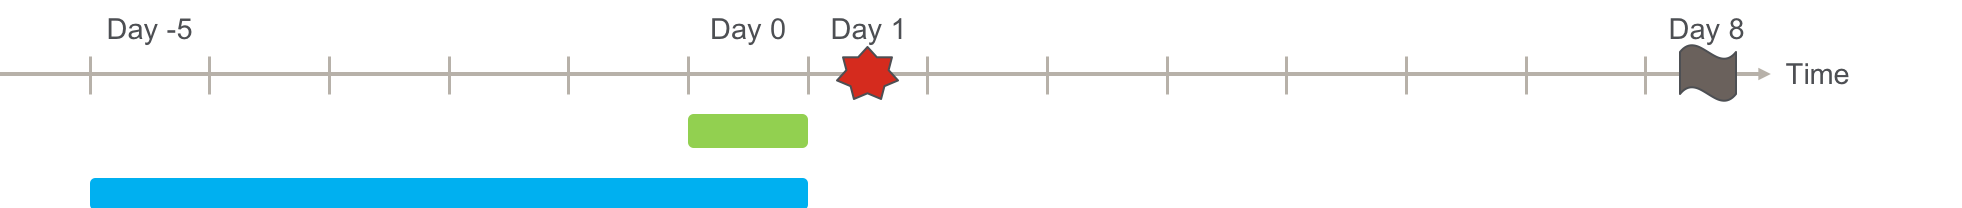
\includegraphics[width=1\linewidth]{timeline}
    \end{center}
    \caption{Graphical representation of the timeline of how the vectors are constructed}
    \label{timeline}
\end{figure}

Figure~\ref{timeline} illustrates how health measurements are collected. On Day\textsubscript{0} as represented by the green Label we collect the data with our 6-hour window averages while from Day\textsubscript{-5} to Day\textsubscript{0} we also aggregate with 1 day windows. On Day\textsubscript{1} we monitor \acrshort{via} calls for potential failure (so that we can, using health measurements collected on Day\textsubscript{0}, predict whether the \acrshort{cpe} will fail the following day). In order to validate our labeling of the problem happening on Day\textsubscript{1} we need to wait Day\textsubscript{9} to make sure that the \acrshort{ftr} flag has been set as we have explained it previously. 

Therefore when collecting the data on a given day $d$, we can collect vectors that have a $\text{Day\textsubscript{0}} = d-1$ (as represented in our \acrfull{plsql} packages by the variable \texttt{var\_day\_0}). We do not flag vectors to determine whether they are failing or not at collection time. Indeed we have only a short history available to construct these vectors. But also we need to wait the \acrshort{ftr} flag to be set before we can label them. Therefore on day $d$, we collect pieces of information that we extract from \acrshort{via} such that for such vectors $\text{Day\textsubscript{0}} = d-8$ (respectively represented by \texttt{var\_via\_day\_0}). We will discuss at a later stage how we can join these two sources.


\subsubsection{Efficiency}
\paragraph{\acrshort{dmp} and \acrshort{dmt}}
As we started developing the project, we used \acrfull{dmp} as a playground but soon enough we were told that this server was to be used only for production-ready software. Indeed there exist a second server dedicated to testing called \acrfull{dmt}. This server, on the other hand, provides much less computational power but also allows us to store any amount of data that we may need to store for the sake of this project. Hence to leverage the power of \acrshort{dmp} and the storage capabilities of \acrshort{dmt} we had to develop a strategy: doing aggregations on the production data mart and storing the results on the test environment.


\paragraph{Rolling Window Mechanism - \acrshort{dmp}}
Our aim was to avoid as much as possible duplicated computation and to efficiently use the resources that are available for the \acrshort{poc}'s development. That's where we derived a rolling window mechanism to iteratively construct the vectors. Put simply, every day we compute the aggregates and wait until we have enough aggregates to build a full vector (which involves computing the differences between aggregate as stated in Section~\ref{subsubsec:time_representation}). 

We have created, on \acrshort{dmp}, four \textbf{buffer tables}. These will temporarily hold data in order to be later assembled into five days vectors:
\begin{itemize}
	\item \texttt{VECTOR}\footnote{We won't state the schema into which we are but for the duration of the \acrshort{poc} all work resided in \texttt{HUMOREAU}.}: holds what we have defined as static information as well as the 6h window averages for the past 24 hours for Day\textsubscript{0} $= \texttt{var\_day\_0}$.
	\item \texttt{DAILY\_AVG\_DAY\_0}: stores the measurements of Day\textsubscript{0} aggregated on a daily basis for all Day\textsubscript{0} $\in \{\text{\texttt{var\_day\_0}}-1,\text{\texttt{var\_day\_0}}\}$
	\item \texttt{DAILY\_AVG\_DIFFS}: stores the daily average differences (except for features that are static, as described in Section \ref{subsec:mes_choices}, that are stored as averages) between Day\textsubscript{0} and Day\textsubscript{-1} for all Day\textsubscript{0} $\in \{\text{\texttt{var\_day\_0}}-4,...,\text{\texttt{var\_day\_0}}\}$
	\item \texttt{VIA\_MACS}: holds the \acrshort{mac}s that have been identified as failing on Day\textsubscript{0}$=\text{\texttt{var\_via\_day\_0}} = \text{\texttt{var\_day\_0}} - 8$. Indeed it holds more details about such \acrshort{mac} that could be useful for future reality checks (\texttt{MAC}, \texttt{DAY\_0}, \texttt{MILESTONE\_NAME}, \texttt{CASE\_ID},\texttt{SESSION\_ID},\texttt{EMP\_ID}, \texttt{CLY\_ACCOUNT\_NUMBER}, \texttt{CASE\_START\_T}, \texttt{PROCESS\_FLOW}, \texttt{FLG\_FTR\_7D\_FLG},\texttt{FLG\_FTR\_0D\_FLG}).
\end{itemize}
Note that each table is uniquely identified by the pair (\texttt{DAY\_0},\texttt{MAC}) which will allow us at a later stage to join these chunks of information. Also note that \texttt{VIA\_MACS} contains information about days that are 8 days earlier than the earliest of the first 3 tables as explained above.

Every day we update the content of these tables in order to always satisfy the four properties we just defined. In order to perform these operations, we have introduced 33 \textbf{intermediary tables} that allow us to temporarily hold computations that are necessary to fill in buffer tables. Their content is purged at the end of each run. Given that the different steps regarding how we fill intermediary tables have been documented and that the general procedure has been explained we didn't judge necessary to explain it in detail here.

To update the content of buffer tables the package will, for Day\textsubscript{0} being the $ \text{\texttt{var\_day\_0}}=\text{current day} - 1$:
\begin{enumerate}
\item Find the static information and compute the 6 hour averages of the chosen measurements over \texttt{var\_day\_0}. Insert them into \texttt{VECTOR}. Delete the entries in \texttt{VECTOR} that correspond to an older day.
\item Aggregate the 6-hour window averages into daily averages. And insert them into \texttt{DAILY\_AVG\_DAY\_0}. It will then also delete the entries in the table that are the eldest (that is entries for which $\text{Day\textsubscript{0}}=\text{\texttt{var\_day\_0}}-2$).
\item Use the daily averages in \texttt{DAILY\_AVG\_DAY\_0} for $\text{Day\textsubscript{0}}=\text{\texttt{var\_day\_0}}$ and $\text{Day\textsubscript{0}}=\text{\texttt{var\_day\_0}}-1$ in order to construct the differences between Day\textsubscript{0} and Day\textsubscript{-1}. It will then insert them into \texttt{DAILY\_AVG\_DIFFS}. Again it will delete the content of the table that is the eldest, that is entries which $\text{Day\textsubscript{0}}=\text{\texttt{var\_day\_0}}-5$.
\item Finally, it fills in the \acrshort{mac}s that have been identified as failing for $\text{Day\textsubscript{0}}=\text{\texttt{var\_day\_0}}-8$ and will delete the old content of the table that is a day older. 
\end{enumerate}

\paragraph{Rolling Window Mechanism - \acrshort{dmt}}
\acrshort{dmt} will hold the tables that store the unloaded versions of \acrshort{dmp} once the vectors have been materialised:
\begin{itemize}
	\item \texttt{VECTOR\_FIVE\_DAYS\_II}\footnote{the suffix of the table indicates it is the second iteration of such table and we will explain why in Section~\ref{subsec:data_sampling}.}: holds all 5 days vectors with the components and representation that were discussed earlier.
	\item \texttt{VIA\_MACS}: holds all the information that is collected in the homonym table created on \acrshort{dmp} for all Day\textsubscript{0} since we started collecting data.
\end{itemize}

Again each table entry is uniquely identified by the pair (\texttt{DAY\_0},\texttt{MAC}). The update that runs every day will happen after \acrshort{dmp} table content has been successfully completed (we should explain how we synchronise between these two tables in the following paragraph). In order to perform the update, the package will:
\begin{enumerate}
	\item Construct a flat vector with the whole content of \texttt{DAILY\_AVG\_DIFFS}, such that for each (\texttt{DAY\_0},\texttt{MAC}) we have the daily average differences of the 5 previous days in a single vector.
	\item Compute the differences between the 6h window averages in \texttt{VECTOR} as explained in Section~\ref{subsubsec:time_representation}. into one vector for each pair (\texttt{DAY\_0},\texttt{MAC}). Prepend each vector with the static information that can also be found in \texttt{VECTOR}.
	\item Finally, it can join everything we have just constructed into a single vector with the daily average for \texttt{DAY\_0} from \texttt{DAILY\_AVG\_DAY\_0} as we desired and insert them in \texttt{VECTOR\_FIVE\_DAYS\_II}.
	\item The last step is to dump all the content of \acrshort{dmp}'s \texttt{VIA\_MACS} into the homonym table in \acrshort{dmt}.
\end{enumerate}

\paragraph{Automatisation: Checks and Logging}
Because these two packages have to be executed daily (even on non-working days) it would be desirable not to have to launch execution manually every time. 

In order to synchronise the two packages, we had to design a way to log events of each procedure. The main challenge is that whenever a procedure fails to update the state of a database then the whole state of the database is rolled back. Therefore we created a logging table (\texttt{LOG\_TABLE} on each data mart). These are updated using autonomous transactions. It means that the transaction itself has independent commit with respect to the rest of the procedure (allowing us to keep a trace of what happened even when the state is rolled back). The behavior of this log table was implemented in \texttt{CPE\_FAILURE\_ERROR\_LOG}. It will contain:
\begin{itemize}[noitemsep]
	\item Execution times of each part of the package.
	\item Insertion counts into intermediary and buffer tables.
	\item Potential errors that happened during execution (either using custom made error messages for expected errors or using \acrshort{sql} error messages)
	\item Flags allowing to know whether the full procedure was successful. 
\end{itemize}		

But to automatise execution we needed a couple of tricks to ensure correctness of collected data. First, each package before being executed respectively on the production and test environment will perform multiple checks:
 \begin{itemize}
	\item \acrshort{dmp}:  \begin{itemize}[noitemsep,topsep=0pt]
					\item Check the state of the database: the correct dates are in the buffer tables w.r.t the Day\textsubscript{0} that will be computed (because it is a rolling window if the past iteration wasn't successful or didn't happen we cannot compute the current one).
					\item Check that the last run performed without errors (by verifying that the log table is empty as it should be emptied by the \acrshort{dmt} package in case of a successful run).
					\item Make sure that intermediary computations yield non-empty results when they shouldn't (it can happen that some table are empty e.g. \acrshort{via} can yield no identified failing \acrshort{cpe}s which shouldn't raise an error).
				\end{itemize}
	\item \acrshort{dmt}: 	\begin{itemize}[noitemsep,topsep=0pt]
					\item Make sure that \texttt{var\_day\_0} is strictly posterior to what we have already computed.
					\item Ensure that the \acrshort{dmp} procedure has executed correctly (if so it will dump the content of the log table in production into test after having reset it).
					\item Again it will make sure that content is indeed inserted when expected (no empty insertion count)
				\end{itemize}
\end{itemize}	

These tricks allowed us to make the two procedures into a job that could be run automatically using SAP and that would send us an email depending on the success or failure of the job. 

\subsection{Data Sampling}
\label{subsec:data_sampling}

Because we decided to keep collecting data as long as we could in order to build a more comprehensive dataset, the size of the original \texttt{VECTOR\_FIVE\_DAYS} table became quickly concerning. Running queries on such a big table\footnote{When it contained 30 days of data, the table had a size of 210 GB, mostly due to the fact that every day we insert 500'000 entries of 291 columns.} was taking prohibitively too much time. 

It was not an option to import the whole constructed dataset on the data analysis machine (a personal computer), first of all, because of its size but also because any way we were going to subsample the healthy class in order to train our models. Therefore we derived a technique to be able to sample from this table easily at the database level. 

Upon insertion we create a \texttt{SEQ\_ID} that is automatically generated by \acrshort{sql} such that it will be incremented at each insertion (what is called an \texttt{AUTO\_INCREMENT} column). Because of some limitation from Oracle, this \texttt{SEQ\_ID} is ensured to be strictly increasing but not necessarily sequential (though it should be very rare that a gap appears between such IDs). By making \texttt{SEQ\_ID} as a key on the table, we can be sure that obtaining entries with a particular value in such field will be done in an optimised way. This is why the table \texttt{VECTOR\_FIVE\_DAYS} has evolved into \texttt{VECTOR\_FIVE\_DAYS\_II}.

In order to sample from the dataset (as implemented in \texttt{SAMPLE} on the \acrshort{dmt} package):
\begin{enumerate}
	\item We join \texttt{VIA\_MACS} with \texttt{VECTOR\_FIVE\_DAYS\_II} in order to obtain the vectors corresponding to unhealthy \acrshort{mac}S.
	\item Then we randomly sample from \texttt{VECTOR\_FIVE\_DAYS\_II} by using a random series of \texttt{SEQ\_ID} ranging on the full range of those\footnote{To make execution faster we decided to tolerate collisions between the healthy and unhealthy \acrshort{mac}s. That means that when the selected sampling size is $n$ we might end up with slightly less than $n$ entries. Nevertheless given the relative small size of the 'sick' class w.r.t. the 'healthy' one, collisions are sufficiently unlikely to be ignored.}. 
	\item We join the two tables that were obtained from the previous steps and insert the result into \texttt{SAMPLED\_VECTOR} residing in the test environment. 
\end{enumerate}

That technique allowed us to efficiently sample the dataset to fully utilise the 'sick' class and subsample the healthy class to facilitate further analysis.

\subsection{Initialisation}
Finally, in order to allow the project to be restarted at a later time, we decided to provide the necessary packages that would allow automatic initialisation of the state of the tables but also the creation of all the tables that are used by the data collection packages. 

Two distinct versions of the \texttt{CPE\_FAIL\_DETECTION\_POC\_INIT} packages addressing the initialisation of the production and test environment. Both versions have in common that they will first create all the necessary tables (including log tables). These additional packages had to be created as a package will not compile if it references tables that do not exist, hence if the initialisation procedure would be in the same package as the data collecting procedures it would be impossible to initialise tables once they have been dropped.

As we have already explained in great details, \acrshort{dmp} package works iteratively as it needs the state of the buffer tables to be initialised. Therefore, once the \texttt{CPE\_FAIL\_DETECTION\_POC\_INIT.INITIALISE} has been executed we still need to run \texttt{CPE\_FAIL\_DETECTION\_POC.INIT}. Together these procedures will initialise the state of \acrshort{dmp} tables such that a call to \texttt{CPE\_FAIL\_DETECTION\_POC.MAIN\_PROC} (the procedure that collects the data) can be done on the same day. 

Each package has been documented inline in order to explain exact steps that must be followed to allow data collection to be restarted in order to ensure the reproducibility but also to support further development of the project.

\vspace{1 \baselineskip} 
This chapter summarises the most important challenge of this project. Lots of effort has been put in data collection. It required to learn more about the company and fight the obscurity around data sources. This whole process had to be implemented in \acrshort{plsql} which represented yet another overhead but was necessary to comply with UPC's data architecture. Data was chosen and represented based on intuitions and advices from different stakeholders in the company. Finally, the process was automatised to facilitate our work but also to ensure knowledge acquired during this phase would be easily transferable for further development. 
\chapter{Data Analysis and Machine Learning}
This chapter will discuss the steps that were followed during the analysis of the collected data. First we should look into the intermediary analysis that was conducted while data was being collected. Then the different data preprocessing steps will be justified and explained. Thirdly, we will present the results and motivation of a clustering attempt on the previously constructed vectors. And finally we will dive into the main matter of failure prediction models. 

\section{Intermediary Analysis}
Data collection required some time before it would produce a relevant dataset. With, on average, 112 failing CPEs\footnote{according to our ground truth} every day we would need some time in order to obtain a balanced dataset of sufficient size.

We leveraged this period of time in order to perform some initial analysis. We were interested in two main topics, first we wanted to determine how much did weekends influence the distribution of vectors, secondly we were interested in an exploratory data analysis that would give us a better understanding of the dataset. 

\subsection{Influence of Weekends on Vectors} 
\label{subsec:influence}
Choices that we did during the dataset's construction frequently needed to be arbitrary, even though they were motivated by network experts. Nevertheless, one of our main concerns was around data seasonality. 

Hopefully some of the seasonality is already being taken care of but there are many sources of such:
\begin{itemize}[topsep=0pt]
	\item \textbf{Over hours of the day}: because all vectors are constructed over the exact same hours, we are confident that they are comparable with respect to such seasonality. 
	\item \textbf{Over period of the year}: according to the HFC support expert, the temperature, as an example, could influence the performance of the network and the range of 'standard' values. Nevertheless, due to evident time restriction this couldn't be evaluated. We could argue that this  effect could be attenuated by considering a training dataset constructed on a limited number of past days to train on period specific patterns. 
	\item \textbf{Over days of week}: metrics of the network are highly dependent on the utilisation of each CPE, this is why we surmise a potential influence of the fact that Day\textsubscript{0} is or not a weekend day.
\end{itemize}

We decided to study the latter as we had the data that could help us get a feeling for such problem. An initial naïve analysis based on single variable hypothesis testing was performed to determine whether each feature displayed some evidence of different sampling distribution using the weekend and weekday populations. Then a more refined test based on bootstrapped energy statistics~\cite{energy_test} was implemented. 

We focused on the vectors composed of Day\textsubscript{0} 6-hour window averaged in relative format\footnote{We only consider the past 24 hours and discard the other days}.

\subsubsection{Naïve Approach: Kolmogorov-Smirnov statistic on 2 samples}
The Kolmogorov-Smirnov (KS) test~\cite{wiki:ks_test} is one of the most standard approaches to perform such test. It allows to test whether two populations are likely to be drawn from two distinct sampling distributions. The test isn't so meaningful in our case given that we are in a multivariate case with our vectors. Nevertheless it offers some interesting initial approach as we could observe features that show the most evidence of different sampling distributions.

We should first define the statistical terms that will be used in the following discussion:
\begin{itemize}[noitemsep,topsep=0pt]
	\item \textbf{Null Hypothesis}~\cite{wiki:null_hyp} ($H_0$): is the hypothesis that the test is trying to reject. Here: the two variables come from identical distributions.
	\item \textbf{Test statistic} ($T$): computed from the data and chosen such that large values of $T$ provide evidence against $H_0$. The observed value of $T$, $t_\text{obs}$ is compared to the distribution of $T$ under the null hypothesis. 
	\item \textbf{Significance level} (e.g. $\alpha = 0.05$): represents the probability of rejecting the null hypothesis when it is true. 
	\item \textbf{Confidence level}: indicating how sure you are of your decision to reject the null hypothesis given the observed test statistic ($CL = (1 -\alpha)\times 100\%$).
	\item \textbf{P-value}~\cite{wiki:pvalue}: $p=P_0(T \ge t_\text{obs})$, where $P_0$ is the probability under the null distribution. \textbf{Low values of $p$ suggest that the null hypothesis is false.} If the p-value is under the significance level, we can reject the null hypothesis for the given confidence level.
\end{itemize}

The KS test can be used either by comparing a given variable to a known distribution or directly by comparing two variables which is how we will use it here as we do not have information regarding the underlying distribution of features. 

The test was initially performed on each feature of the feature space which wasn't correct. Indeed, it is designed to be used on continuous distributions. Many features are discrete as for example the \texttt{MISS\_*}. 

Running the test on all continuous features, we focused our attention on features that yielded the lowest p-value as this should be the features for which we are the most confident on rejecting the null hypothesis. 

\begin{table}[h]
\begin{center}
\begin{tabular}{c r r}
\hline
\textbf{Feature} & \textbf{$t_\text{obs}$} & $p$\\ 
\hline\hline
\texttt{CER\_UP\_12H} & $0.128066$ &	 $2.547019\times 10^{-198}$\\
\hline
\texttt{CER\_UP\_6H} &  $0.094043$ & $3.869613\times 10^{-107}$\\
\hline
\texttt{CER\_DN\_18H} & $0.092828$ &	 $2.120185\times 10^{-104}$\\
\end{tabular}
\end{center}
\caption{\label{CPEMes}Features at the CPE level}
\end{table}

\begin{figure}[ht]
    \begin{center}
    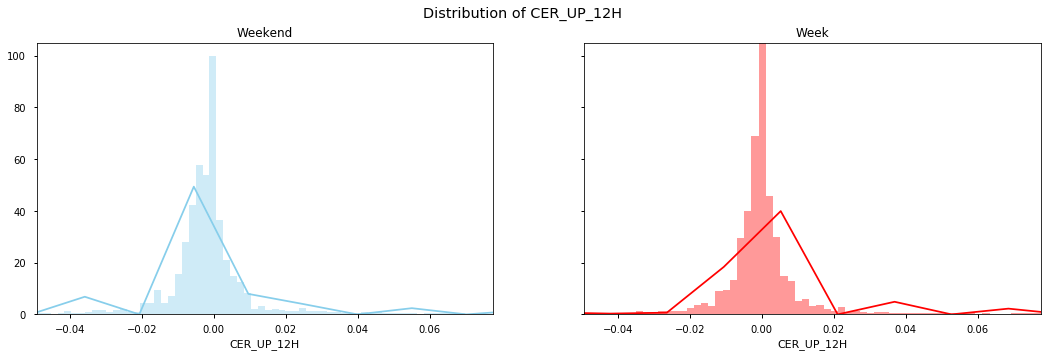
\includegraphics[width=1\linewidth]{images/KS_CER_UP_12.png}    
    \end{center}
    \caption{Comparison of distributions between the weekend and weekday population for \texttt{CER\_UP\_12H}}
    \label{KS_CER_UP_12}
\end{figure}

\begin{figure}[ht]
    \begin{center}
    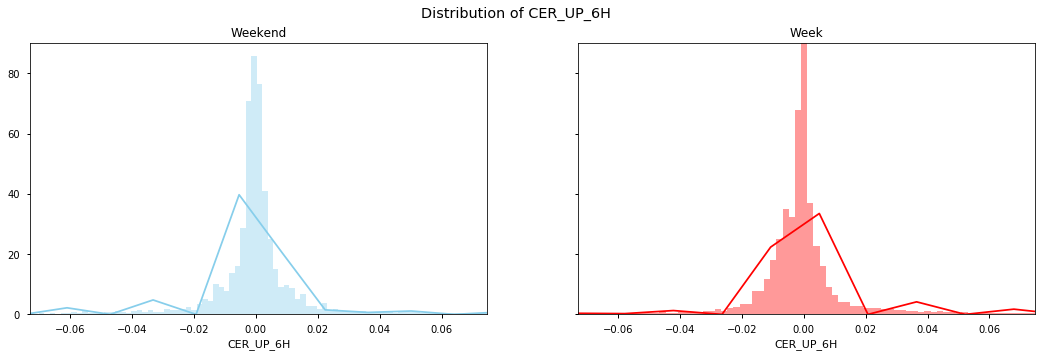
\includegraphics[width=1\linewidth]{images/KS_CER_UP_6.png}    
    \end{center}
    \caption{Comparison of distributions between the weekend and weekday population for \texttt{CER\_UP\_6H}}
    \label{KS_CER_UP_6}
\end{figure}

\begin{figure}[ht]
    \begin{center}
    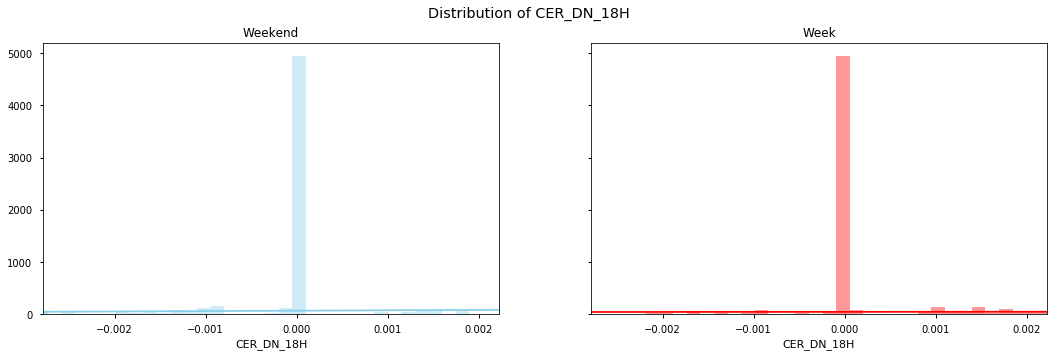
\includegraphics[width=1\linewidth]{images/KS_CER_DN_18.png}    
    \end{center}
	\caption{Comparison of distributions between the weekend and weekday population for \texttt{CER\_DN\_18H}}
    \label{KS_CER_DN_18}
\end{figure}

\begin{figure}[ht]
    \begin{center}
    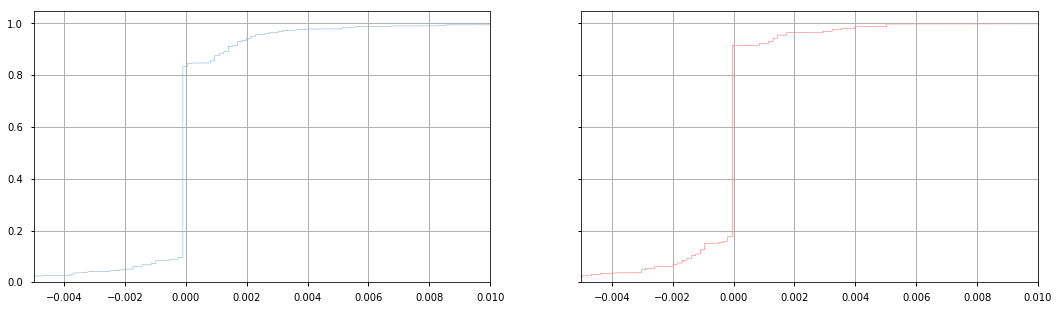
\includegraphics[width=1\linewidth]{images/KS_CER_DN_18_CUMUL.png}    
    \end{center}
    \caption{Comparison of distributions between the weekend and weekday population for \texttt{CER\_DN\_18H} using cumulative distributions (the left curve representing the weekend population)}
    \label{KS_CER_DN_18_CUMUL}
\end{figure}

Figures~\ref{KS_CER_UP_12} and \ref{KS_CER_UP_6} show the distribution of the top 2 p-values. It isn't so obvious from a graphical perspective that these two variables are sampled from different distributions even if we can see that during the week the two features are more likely to be zero (as indicated by the high bar centered in 0 on the right plots). 

For the third feature, the initial plot (cf. Figure~\ref{KS_CER_DN_18}) was not very informative, therefore we decided to switch to a cumulative distribution plot. Again figure~\ref{KS_CER_DN_18_CUMUL} doesn't show much evidence of the two underlying distributions being different.

This concluded our introductory analysis using the KS test. Apparently we cannot show evidence of the two distributions being drastically different. This motivated us to switch to a different test. 

\subsubsection{High Dimensionality Hypothesis Testing}
The previous test, put aside the fact that it wasn't very conclusive, only takes into consideration each individual feature. We are indeed interested in knowing whether the vectors differ between weekend and weekdays. 

High dimensional computation is one of the challenges that is still at the center of research and we studied many papers~\cite{min_energy,two_sample_equality,dimensional_object,energy_test} to determine a proper test to use in our use case. The energy test based on bootstrapped test-statistic estimation seemed promising as it would help us efficiently run such tests.

\paragraph{Theoretical Concept}  
Suppose that we have $X_{1},...,X_{n_1}$ and $Y_{1},...,Y_{n_2}$ independent random samples of random vectors in $\mathbb{R}^d$. Let $\mathcal{A}$ and $\mathcal{B}$ be two populations of samples of respective size $n_1$ and $n_2$ such that $n=n_1+n_2$. The article proposes a new test statistic, the energy:

\begin{align}
	\mathcal{E}_{n_1,n_2} = e(\mathcal{A},\mathcal{B}) = \frac{n_1 \times n_2}{n} ( & \frac{2}{n_1\times n_2} \sum_{i=1}^{n_1}\sum_{m=1}^{n_2}||X_i-Y_m||\\ 
	&- \frac{1}{n^2}\sum_{i=1}^{n_1}\sum_{j=1}^{n_1}||X_i-X_j||\\ 
	&- \frac{1}{n^2}\sum_{i=1}^{n_2}\sum_{j=1}^{n_2}||Y_i-Y_j||)\\
\end{align}

Suppose that $X,X',Y,Y'$ are independent random vectors of $\mathbb{R}^d$ with finite expectations such that $X \buildrel d \over = X'$ and $Y \buildrel d \over = Y'$, then:

\begin{equation}
	2 E||X-Y||- E||X-X'||- E||Y-Y'|| \ge 0
\end{equation}

and the equality holds if and only if X and Y are equally distributed. Therefore we expect the energy statistic to be large if the null hypothesis can be rejected.

\paragraph{Practical Implementation}
Let $\alpha$ be the significance level. We will sample B bootstrap samples $W_1^{(b)},...W_n^{(b)} \quad \forall b \in \{0,...,B\}$ such that $(B+1)\alpha$ is an integer. $W$ is the random variable obtained by sampling from a $X$ and $Y$ with respective probabilities\footnote{This means that we pool all the elements of $X$ and $Y$ in a single set and sample uniformly at random from this set.} $n_1/n$ and $n_2/n$. 

For each bootstrap sample $b$, we compute $\mathcal{E}_{n}^{(b)}$ determined by k samples:

\begin{equation}
\begin{cases}
	\mathcal{A}_1^{(b)} = \{W_1^{(b)},....W_{n_2}^{(b)}\}\\
	\mathcal{A}_2^{(b)} = \{W_{n_1 + 1}^{(b)},....W_{n}^{(b)}\}
\end{cases}
\end{equation}

Then the bootstrap estimate of $P_n(\mathcal{E}_{n} \le t)$ is $\frac{1}{B} \sum_{i=1}^B I(\mathcal{E}_{n}^{(b)} \le t)$.

Put in simple words, we will compute the energy statistic for the original population segmentation giving us $t_\text{obs}$. Then $B$ times, we will create two new populations by sampling from the pooled population. On each bootstrap we will compute the energy bootstrap estimate. We will then check the ratio of bootstrap estimates that are lower than $t_\text{obs}$, this will give us the p-value. 

Because we will compute the distance between two vectors of the pooled population many times, we will start by computing the distance matrix that provides the distance between any two pair of vector from the pooled population.

\paragraph{Results}
The dataset used for this test was composed of 44,556 samples from the weekday population against 17,740 for weekends, therefore the distance matrix would be composed of 790,423,440 entries, which isn't easy to work with on a personal computer due to memory requirements. We derived three strategies in order to perform the test:
\begin{itemize}
	\item \textbf{Averaging vectors over day type}: we average for each MAC the vector over all vectors from the weekend and then all vectors from the week. This provides two populations of equal sizes where there is a single entry per MAC in each.
	\item \textbf{Sampling populations}: we sample from each population without replacement in order to obtain smaller populations. 
	\item \textbf{Multiple samples}: in order to obtain a better estimate we run the previous strategy on ten different samples. This will give us 10 different p-values that we can average to obtain a stronger estimate.
\end{itemize}

\begin{table}[h]
\begin{center}
\begin{tabular}{c r r r l}
\hline
\textbf{Strategy} & \textbf{Observed} & \textbf{Limit} & \textbf{p-value} & \textbf{Decision}\\ 
\hline\hline
Day type average &  $87340.19$ & $71.00$ & $0$ & Reject $H_0$\\
\hline
Subsampling &  $57526.91$ & $86.97$ & $0$ &  Reject $H_0$\\
\hline
Repeated subsampling &  (avg)$58771.53$  & (avg)$100.12$ & $0$ &  Reject $H_0$\\
\end{tabular}
\end{center}
\caption{\label{hyp_test_res}Energy test results for different strategies}
\end{table}

Table~\ref{hyp_test_res} presents the result obtained with this test. The results show that we can reject the null hypothesis at confidence level $>99.99\%$. Therefore we are confident that weekend and weekday's vectors have distinct underlying distributions. To increase our confidence in the test we performed the same test but this time by using two populations generated from exclusively weekday/weekend populations. We expect these tests not to reject the null hypothesis at reasonable confidence levels.

\begin{table}[h]
\begin{center}
\begin{tabular}{c r r r l}
\hline
\textbf{Strategy} & \textbf{Observed} & \textbf{Limit} & \textbf{p-value} & \textbf{Decision}\\ 
\hline\hline
Subsampling (week only) &  $21.15$ & $182.55$ & $0.9394$ & Cannot reject $H_0$\\
\hline
Subsampling (weekend only) &  $18.99$ & $79.40$ & $0.7374$ & Cannot reject $H_0$\\
\hline\hline
Repeated subsampling (week only) & (avg)$32.49$ & $130.61$ & $0.6929$ & Cannot reject $H_0$\\
\hline
Repeated subsampling (weekend only) & (avg)$34.83$ & $76.463$ & $0.4363$ & Cannot reject $H_0$\\
\end{tabular}
\end{center}
\caption{\label{hyp_test_control}Energy test results for control experiments}
\end{table}

Table ~\ref{hyp_test_control} shows that the test doesn't reject the null hypothesis when we are sampling for each distinct population which increases our confidence in results. 

\vspace{1\baselineskip}A preliminary step was followed to mitigate this phenomenon. We constructed for each vector a categorical variable \texttt{WEEKDAY}. It gives us the information regarding what day of the week is Day\textsubscript{0}. It is important to note that "data cannot prove correctness of a theory (hypothesis), because we can always imagine that future data or a new experiment might undermine it, but data can falsify a theory"\footnote{As presented in the "Probabilities and statistics" class given by Pr. Davison (slide 348 of the course book).}. We cannot prove that the two distributions here are different, we can only reject that they are identical at a particular confidence level. 

\subsection{Exploratory Data Analysis}
EDA allows us to gain insights on the data that we are working with. Our problem makes such analysis complex as we are working with 290 features. We decided to only look at particular characteristics of the dataset. We started with a standard data report to understand the distribution of features. We followed with an analysis of the NULL values. Finally, we investigated the correlation among components to ensure that we discard components that do not add value. 

\subsubsection{Data Report}
With 291 components in our vectors, it would have been quite repetitive to produce meaningful plots for each of them. Hopefully the data science team has developed a tool that produces such exploration automatically. In the appendix~\ref{sec:continuous} and~\ref{sec:categorical} we have provided some plots constructed by this package. 

The number of such plot prevents a comment for each of them but we would like to make a few remarks:
\begin{itemize}[noitemsep,topsep=0pt]
	\item Many features are highly skewed in their center, which could be explained by the fact that we expect signal values not to fluctuate too much and therefore the relative difference between two consequent aggregates is expected to be close to zero.
	\item Most features that are not from the \texttt{MISS\_*} type are approximately normally distributed. 
	\item The \texttt{SEQ\_ID} is approximately uniform which supports our confidence in this sequence number to be rarely forming gaps as we argued in section~\ref{subsec:data_sampling}.
\end{itemize}

The report also performed some other analysis but it wasn't particularly relevant due to the size of vectors. As an example a graphical correlation analysis would be unusable here. Hence we performed it in another way. 

\subsubsection{Null Value Analysis}
As we previously mentioned it in section~\ref{subsubsec:constructed_features}, missing values carry a lot of sense for us. Because we have aggregated the data at the database level, we are forced to perform this analysis on the aggregated measurements. This means that we are not necessarily showing the true underlying patterns. 

Indeed, an aggregate is null if and only if all the aggregated measurements are also null\footnote{By design of Oracle's average function that ignores missing values.}. Also the relative difference between two values is null if one of the two components at least is null itself. 

In order to give a high-level view of null values we used a package that allows us to produce a graphical representation of null values. Figure~\ref{white_matrix} illustrates the existence of patterns in missing values. Given the number of columns it is complex to analyse such pattern with that particular graph. 


\begin{figure}[ht]
    \begin{center}
    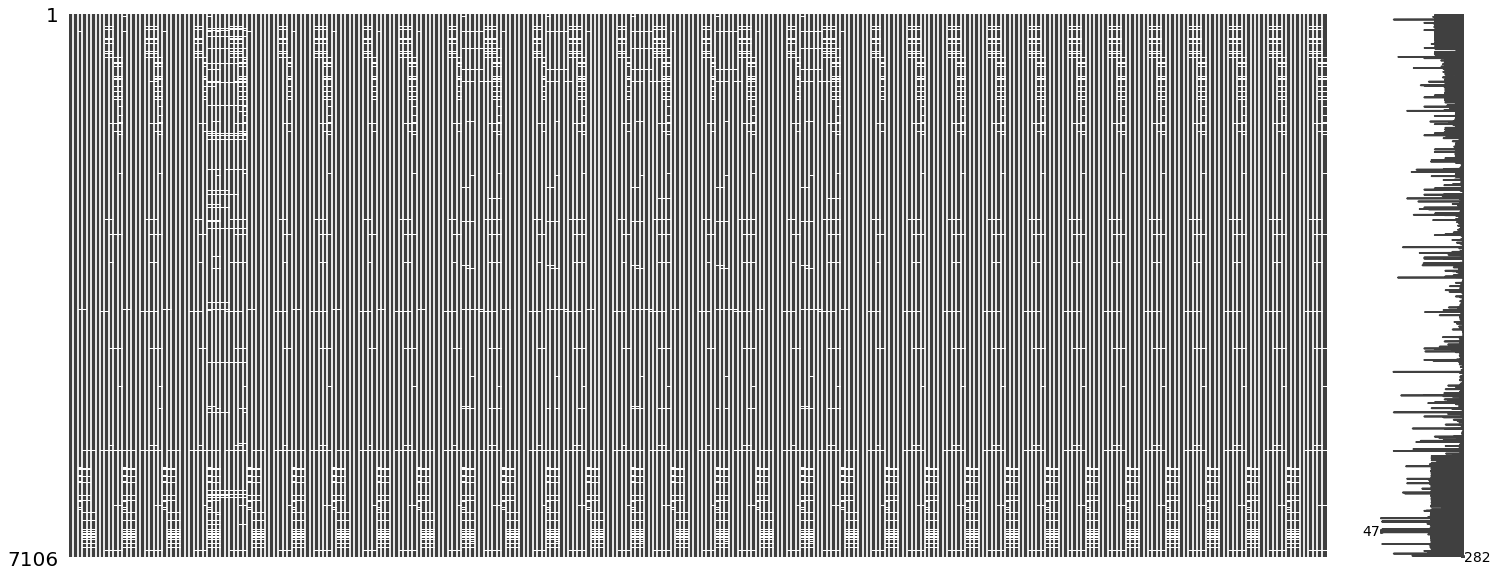
\includegraphics[width=1\linewidth]{null_white_pattern}
    \end{center}
    \caption{Matrix representing missing values as white cells on the dataframe}
    \label{white_matrix}
\end{figure}

We therefore used a dendogram. It displays variable completion, revealing trends deeper than the pairwise ones visible in a correlation heat map. Cluster leaves which are linked together at a distance of zero fully predict one another's presence: one variable might always be empty when another is filled, or they might both be always filled or both empty, and so on.

\begin{figure}[ht]
    \begin{center}
    
\includegraphics[width=1\linewidth]{dendogram_part}
    \end{center}
    \caption{Data completion dendogram (partial)}
    \label{dendogram}
\end{figure}

As the graph is too long to fit on a page, only a fraction of it is presented in the figure~\ref{dendogram}. What is interesting is to see that measurements are grouped by days at which they are aggregated but also sometimes by the fact that they are taken at the CMTS or CPE level. 

Regarding the level of collection of the data, this data completion correlation could indicate some data polling issues on particular period of time. Also the fact that multiple measurements have data completion correlation when computed on the same time window could confirm the intuition that measurements are most probably missing when the CPE is offline. 

This analysis only gives coarse grain patterns as it would be complicated to look at every single clustering to determine some underlying pattern. Therefore we moved to a correlation analysis on the feature space not only taking into account data completion. 

\subsubsection{Feature Elimination}
By analysing highly correlated variables our aim was to reveal features that do not add much usable information for further works and could be discarded. Then we also decided to determine whether some component of the vector was particularly inexpressive. 
 
\paragraph{Correlated Features}
As we started the correlation analysis, we discovered that some features were exactly identical for every single sample. This proved to be a mistake during the data collection process. For the \texttt{MISS\_*} features, we have added two features, namely \texttt{MISS\_\{mes\}} and \texttt{MISS\_\{mes\}\_1d} that both represented the ratio of missing values over the past day. Hopefully this could easily be fixed by deleting the duplicate when importing the data (correcting the data collection package would have invalidated all data collected so far so we decided to prefer a fix at import time).

Once this was fixed, we could look at highly correlated features. This revealed 48 groups of features that had a correlation higher than $0.9$. We split these groups in two. First, those that correspond to two or more measurements that are correlated for every single time aggregate. This is most likely showing that original measurements are correlated. That yielded 4 groups of correlated measurements:
\begin{itemize}[noitemsep,topsep=0pt]
	\item \texttt{CMTS\_MS\_UTILIZATION\_UP} $\equiv$ \texttt{CMTS\_UTILIZATION\_UP}
	\item \texttt{MISS\_PCT\_TRAFFIC\_SDMH\_UP}  $\equiv$ \texttt{MISS\_PCT\_TRAFFIC\_DMH\_UP}
	\item \texttt{MISS\_SNR\_DN}  $\equiv$ \texttt{MISS\_RX\_DN}  $\equiv$ \texttt{MISS\_TX\_UP}
	\item \texttt{MISS\_SNR\_UP}  $\equiv$ \texttt{MISS\_RX\_UP}
\end{itemize}
In order to decide whether we could discard all but one feature of each of these groups, we plotted for each time aggregate each measurement of the correlation group against each other. For each group these plots displayed strong evidence that the measurements are nearly identical but also Pearson and Spearman correlations were always above $0.98$. Therefore we always discarded all measurements but one from the correlation group in order to discard measurements that would not add information. Table~\ref{correlation_insp} only presents such plot for the first group of variables, for other groups the results can be found in the final notebook and are similar to the one we chose to display.

\begin{figure}[h]
\begin{center}$
\begin{array}{ccc}
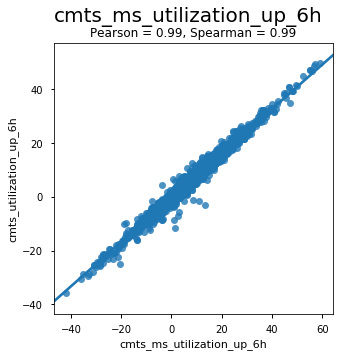
\includegraphics[width=1.5in]{correlation-1} &
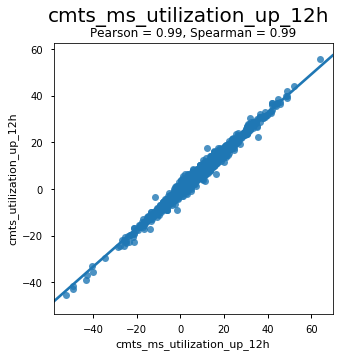
\includegraphics[width=1.5in]{correlation-2} &
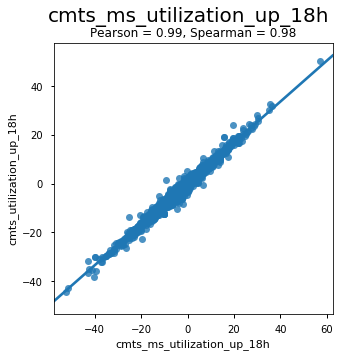
\includegraphics[width=1.5in]{correlation-3}\\
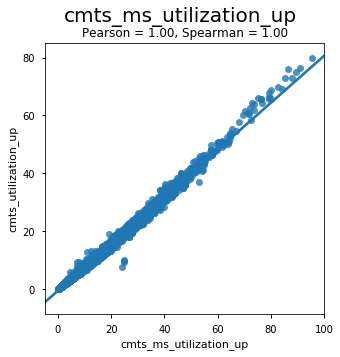
\includegraphics[width=1.5in]{correlation-4} &
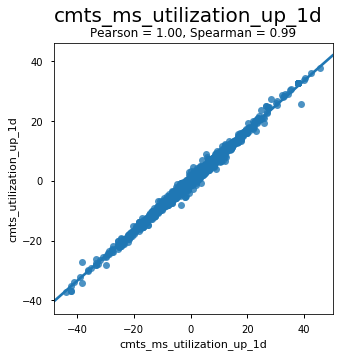
\includegraphics[width=1.5in]{correlation-5} &
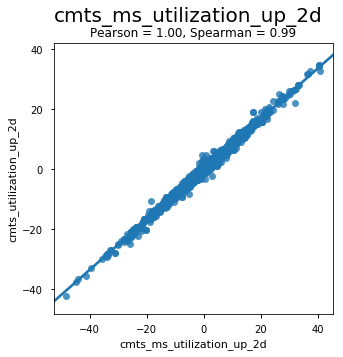
\includegraphics[width=1.5in]{correlation-6}\\
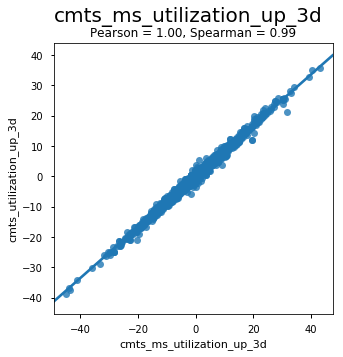
\includegraphics[width=1.5in]{correlation-7} &
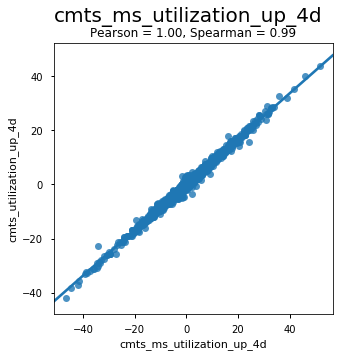
\includegraphics[width=1.5in]{correlation-8} &
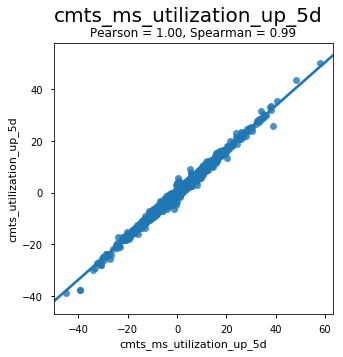
\includegraphics[width=1.5in]{correlation-9}\\
\end{array}$
\end{center}
\caption{\label{correlation_insp}Graphical correlation inspection for \texttt{CMTS\_MS\_UTILIZATION\_UP} $\equiv$ \texttt{CMTS\_UTILIZATION\_UP}}
\end{figure}

Then we investigated 3 groups of features that were not correlated for every time aggregate:
\begin{itemize}[noitemsep,topsep=0pt]
	\item \texttt{MISS\_RX\_UP\_24H} $\equiv$ \texttt{OFFLINE\_PCT\_24H}
	\item \texttt{MISS\_RX\_UP\_6H}  $\equiv$ \texttt{OFFLINE\_PCT\_6H}
	\item \texttt{MISS\_SNR\_DN}  $\equiv$ \texttt{MISS\_RX\_UP}
\end{itemize}
Figure~\ref{almost_correlation_insp} shows scatter plots (using hex bins to show density at particular points) of each feature plotted against the one that it seems correlated to. We see that some correlation pattern exists. Nevertheless we decided not to discard any of these features. Indeed, graphical correlation isn't as explicit but also because the correlation on particular time aggregates doesn't explain a correlation at the raw measurement level. These particular cases could be handled either by the model that will not use the features or by a dimensionality reduction techniques at a later stage.

\begin{figure}[h]
\begin{center}$
\begin{array}{ccc}
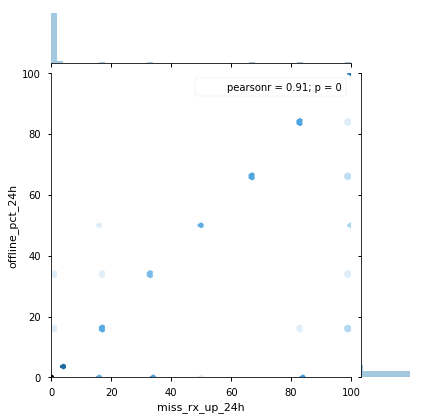
\includegraphics[width=2in]{almost_corr_1} &
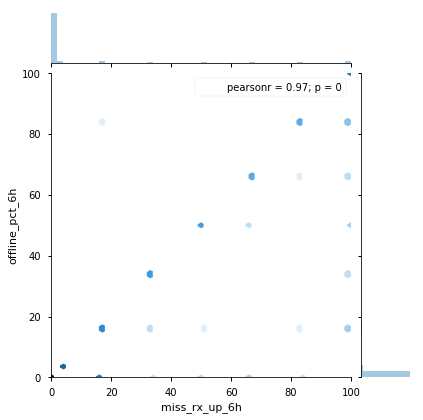
\includegraphics[width=2in]{almost_corr_2} &
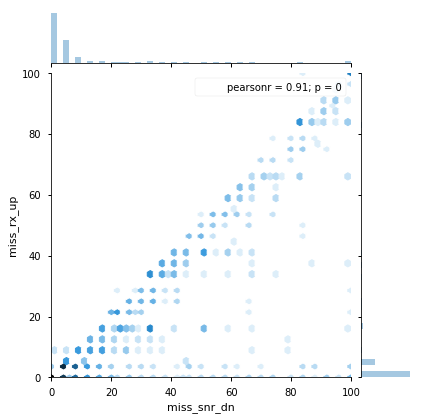
\includegraphics[width=2in]{almost_corr_3}
\end{array}$
\end{center}
\caption{\label{almost_correlation_insp} Graphical correlation inspection for features that are not correlated for every time aggregate}
\end{figure}

\paragraph{Near Zero Variance}
By inspiration from the R package called caret\footnote{\url{https://www.rdocumentation.org/packages/caret/versions/6.0-80/topics/nearZeroVar}}, we also investigated features that do not have much variance. To detect such features we focused on those that satisfy any of the following two characteristics:
\begin{itemize}[noitemsep,topsep=0pt]
	\item The most common value is represented by more than 99\% samples (near zero variance predictors)
	\item Very few unique values w.r.t the number of samples (by default $<10\%$) and the frequency of the most common value to the frequency of the second most common value is large (by default $>95/5$)
\end{itemize}

Figure~\ref{nearzerovar} presents the features that we investigated. As we should explain in Section~\ref{sec:datapreprocessing}, \texttt{model\_i} are features that encode the \texttt{HARDWARE\_MODEL} and therefore for such variables we expect low variance. Other variables are discrete and therefore as a second intuition we wondered if by discarding these features we would not be shaving off exactly the features that give us outliers. Some graphical investigation seems to indicate that most of these features were flagged du to the high skew in their center as we already witnessed it in the data report. This investigation yielded no interesting results. 

\begin{figure}[ht]
    \begin{center}
    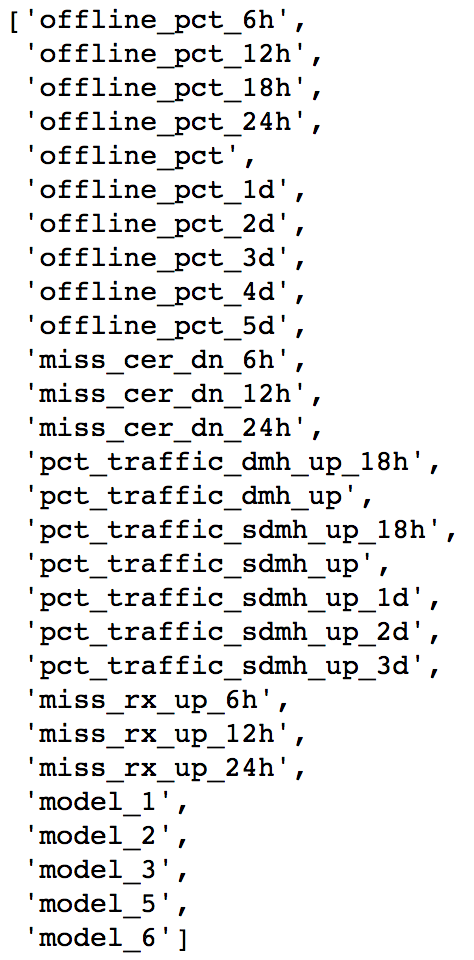
\includegraphics[scale=0.5]{nearzerovar}
    \end{center}
    \caption{Features flagged by the \texttt{NearZeroVar} function (suspected of having low variance)}
    \label{nearzerovar}
\end{figure}

\vspace{1\baselineskip}
The intermediary analysis allowed a better grasp of the characteristics of the dataset. Thanks to a high-dimensional test we determined that weekends had an influence on vectors and tried to mitigate this influence by adding a new feature. Then we explored our dataset to find out about the distribution of features as well as their correlation. 

\section{Data Preprocessing}
\label{sec:datapreprocessing}
Data preprocessing steps are necessary for most of models to perform well. We will discuss the different strategies that have been used in order to preprocess the dataset for classification. In the following paragraphs we will consider $x_i^{(1)},...,x_i^{(d)} \quad \forall i\in \{1,...N\}$ (number of samples) and  $\forall d \in \{1,...D\}$ (dimension of each sample) to be our input and $y_i \quad \forall i\in \{1,...N\}$ to be our target. Finally we will denote by $\hat{y}_i \quad \forall i\in \{1,...N\}$ the predictions of our model.

\subsection{Target Binarization}
At the start of the project we considered the possibility of performing a multi-class classification. This explains our attention to the correctness of labels. That would allow to achieve other business goals as providing a new tool to diagnose CPE problems and automatically determine the good flow to service the customer. Nevertheless, an initial approach would be to start with a binary classification. Therefore rather than focusing on labels we would focus entirely on whether the CPE is failing or not (which we indicate by transforming the \texttt{MILESTONE\_NAME} feature into 1 and 0 to indicate if it is respectively sick or not.
 
\subsection{One-Hot Encoding}
\label{subsec:one_hot}
As described by the collaborative encyclopedia~\cite{wiki:onehot}, one hot encoding allows to describe a categorical feature by creating as many features as there are categories and setting exactly one feature to the high state (1) when the original feature lies in this particular category. This is a desirable modification as some models heavily relies on the value of a particular feature. In our case we have two categorical features \texttt{WEEKDAY} and \texttt{HARDWARE\_MODEL}. 

If we consider a simple linear regression, it will compute a weight $\omega_i^{(k)}$ to each feature $x_i^{(1)},...,x_i^{(d)}$ such that $\hat{y}_i=\sum_{k=1}^d{\omega_i^{(k)}\times x_i^{(1)}}$ (the linear combination determines the predicted label). Hence one can see that for a categorical feature as \texttt{WEEKDAY} it wouldn't make sense to care about its absolute value but rather what is the value it takes. Hence we created two new groups of features \texttt{wk\_\{i\}} and \texttt{model\_\{i\}}.

\subsection{Missing Value Imputation}
Because a machine learning algorithm works with an underlying mathematical model it requires numbers to perform correctly. This is why we need to transform missing values. There exist many imputation techniques, nevertheless in our case we do not need too much reflexion regarding the one to use. Indeed, as we discussed in section~\ref{subsubsec:constructed_features}, we have added a feature that provides the information of missing values such that we do not lose it. 

Our aim is to "hide" missing values as well as we can. Because of our scaling choice that we should discuss in next subsection we will replace each missing value by the feature's mean.


\subsection{Scaling}
This addresses the same problem as discussed in section~\ref{subsec:one_hot}. We wish features to have comparable scales in order to not bias our models toward a particular feature importance consideration. This is not necessary for each model but it is desirable to apply it for model exploration to be able to black box test each model. We will discuss later on its usefulness for our picked models. 

\begin{table}[h]
\begin{center}
\begin{tabular}{c c p{80mm}}
\hline
\textbf{Strategy} & \textbf{Scaled Features} & \textbf{Comment} \\ 
\hline\hline
Log Scaling & $x_i'=\log(x_i)$ & Good for heavy tailed features (Distribution with higher probability of getting large values)\\
Min-Max Scaling & $x_i' = \frac{x_i - min}{max-min}$  & May scale typical values to small intervals in case of outliers\\
Standardisation & $x_i' = \frac{x_i - \mu_i}{\sigma_i}$ & Very meaningful in case of normally distributed features and more resistant to outliers. (Where $(\mu_i, \sigma_i)$ are the mean and standard deviation of the feature)
\end{tabular}
\end{center}
\caption{\label{scaling}Scaling strategies}
\end{table}

Out of the three main strategies that we considered and presented in table~\ref{scaling}, we decided to standardise features. This is coherent with the data report that displays many normally distributed features but also because many features contain outliers.

\subsection{Dimensionality Reduction}
The curse of dimensionality~\cite{wiki:curse} is an important problem in cases that are similar to ours. Indeed, we are here working with many features and as many models rely on the notion of distance they might be ineffective due to meaninglessness of such notion in high-dimensional spaces (which is also why we had to use specific techniques in section~\ref{subsec:influence}).

To fight high dimensionality of the feature space different techniques exist and we experiment with two of them.

\subsubsection{Principal Component Analysis}
PCA is a popular dimensionality reduction technique~\cite{pca} that compresses the data to display it in a more meaningful representation which relies on the use of singular vector decomposition. It can be sometimes misleading as we often talk about PCA's number of components used. These components should not be confused with features, these are rather the number of vectors that will compose the new base to represent our data. 

\begin{figure}[ht]
    \begin{center}
    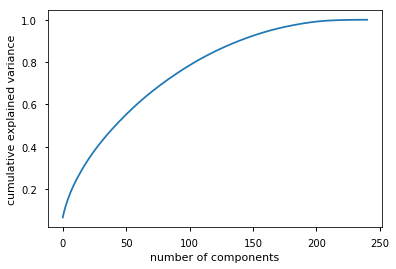
\includegraphics[scale=0.5]{pca_var}
    \end{center}
    \caption{Tradeoff between the level of variance explained and the number of components of PCA}
    \label{pca_var}
\end{figure}

Figure~\ref{pca_var} illustrates how by considering an increasing number of components we increase the cumulative explained variance. To leverage the power of PCA's compression we decided to retain 95\% of the variance with PCA. Again this could be more finely tuned but was chosen as a baseline. 

\subsubsection{Linear Discriminant Analysis}
LDA~\cite{wiki:lda} uses an extra piece of information. It uses the labels of samples in order to find a single number combination of features that separates the most classes. The resulting combination can be used already as a linear classifier but is most commonly used solely as a dimensionality reduction technique. Because it gives weight to each feature, it may not be necessary to scale them beforehand. 

\vspace{1\baselineskip}
The first two preprocessing steps, Binarization and one hot encoding are grouped together as they are performed on all samples of the dataset. On the other hand, dimensionality reduction, imputing and scaling have to compute statistics on the training set that are applied both on the training and testing set. Therefore they need to be done when the model is fitted/train and will be grouped with the classifier. For the purpose of efficient implementation, we used a component proposed by scikit-learn called pipeline\footnote{\url{http://scikit-learn.org/stable/modules/generated/sklearn.pipeline.Pipeline.html}}. It allows to group different steps into a single object that can then be used as black box for the ML part. 

\section{Clustering Attempt}
Considering some of the characteristics of the way that we label our samples we thought that clustering coupled with some expert help at analysing these clusters would help us enhance labeling. Indeed, customer calls cannot be considered as the strongest indicator of whether a particular CPE is failing. This is due to multiple reasons. First of all, we cannot be sure that every customer has the same way of dealing with CPE failures. Some might call the service center in the following minutes because they are using the service at the moment of failure, some may fix the problem themselves by rebooting the CPE or some other quick fix. Hence we cannot be sure that a particular problem will be flagged in the same timeframe than another instance of that problem, or that it will be flagged at all. Secondly, we used a database that was not designed to answer this project's requirements and therefore we had to filter down the data and may be discarding many 'sick' CPEs for the sake of problem labeling precision. 

Therefore by clustering our vectors we aimed at unveiling the underlying structure that would indicate failures. In the case where we would have found a clustering displaying satisfying structure we could have gone to Jonas Staempfli in order to look with him at the CPEs that are grouped together to determine.

In this section we will present the different methods that have been tested to cluster the data, then we will discuss the result of such clustering and try to explain why we think it isn't usable.


\subsection{Exploring}
We started with the most popular and simple model: K-Means clustering. Many clustering algorithm exist but often require to tune multiple parameters in order to obtain decent results which motivated our choice of the simplest clustering algorithm.

\subsubsection{Evaluating Performance}
Because clustering is unsupervised it is usually difficult to evaluate its performance. In our case, we do have the labeling but are interested in improving such labeling forcing us not to rely entirely on it. Extending our existing labeling by propagating labels inside clusters based on majority votes could lead to a serious overestimation of the performance of a future classifier (it would be as if we decided to change the labels of samples that are classified as false negatives or false positives such that they are now classified correctly).

\paragraph{Silhouette Analysis}
A silhouette analysis is used to assess the structure of a clustering. It uses a measure that translates how close each point in one cluster is to points in the neighbouring clusters. This measure ranges in $[-1,1]$ and is called a \textbf{silhouette coefficient}. 

Silhouette coefficients close to 1 indicate that the sample is far away from the neighbouring clusters. A value of 0 indicates that it lies on the decision boundary between two clusters and a value near -1 indicates that the sample might have been assigned to the wrong cluster.

Using these coefficients, we can decide on the most appropriate hyper-parameter like $k$ (number of clusters) in our case. We create plots were we show ordered coefficient values for all points in each cluster. The interpretation of such plot resides in the fact that:
\begin{itemize}
	\item we wish to avoid having certain cluster that have below average silhouette scores (as indicated by the red line)
	\item we wish to have homogeneous size in the silhouette plots (when the classes are supposed to be balanced, which is a basic assumption of K-Means)
\end{itemize}

But also we can use the average of silhouette coefficients in order to determine the quality of the model~\cite{silhouette}:
\begin{itemize}[topsep=0pt,noitemsep]
	\item $[1.0,0.7)$ : A strong structure has been found
	\item $[0.7,0,5)$ : A reasonable structure has been found
	\item $[0.5,0.25)$ : The structure is weak and could be artificial. Try additional methods of data analysis
	\item $< 0.25$ : No substantial structure has been found
\end{itemize}

\paragraph{Elbow Method}
Another method that we tried to use was the elbow method. It uses a plot of the Sum of Squared Error (SSE) against the number of clusters to determine the optimal $k$. The point where the plot starts flattening significantly (forming an elbow) indicates the optimal number of clusters. 

\subsubsection{Initial Results}
Using only preprocessing (scaling and imputation), we used a sample of the data that was collected up to the 27\textsuperscript{th} in order to attempt to cluster. 

\begin{table}[h]
\begin{center}
\begin{tabular}{c c c}
\hline
\textbf{$k$} & \textbf{(Scaling+Imputing)} & \textbf{(+PCA)}\\ 
\hline\hline
2 & \textbf{0.2837} & \textbf{0.4354}\\
3 & 0.0235 & 0.0928\\
4 & 0.1524 & 0.2033\\
5 & 0.0112 & 0.0636\\
6 & 0.0120 & 0.0160\\
7 & 0.0219 & 0.0491\\
\end{tabular}
\end{center}
\caption{\label{silh_scor_simple}Average silhouette scores for different number of clusters with scaled and imputed data}
\end{table}

\begin{figure}[ht]
    \begin{center}
    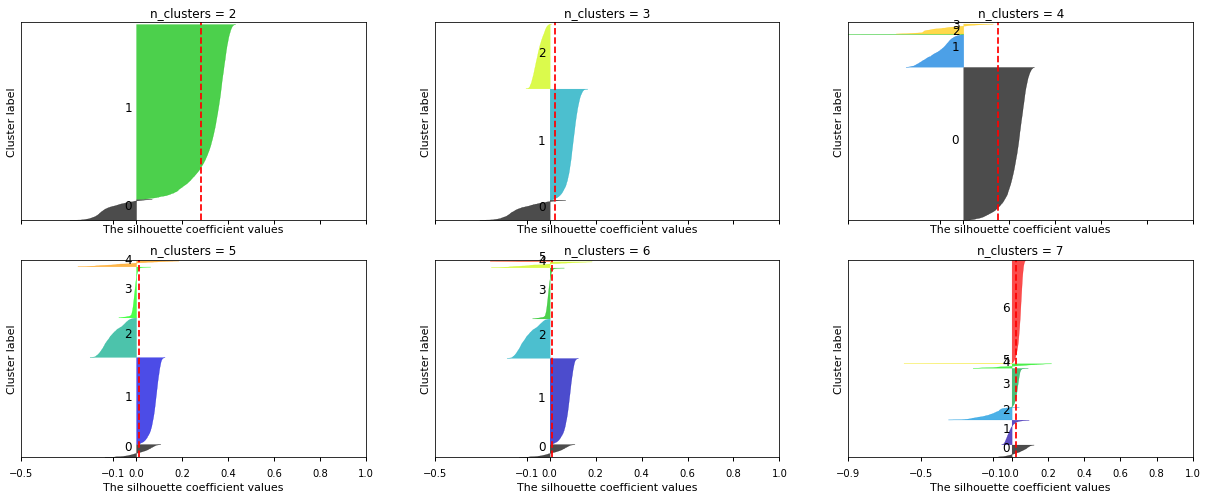
\includegraphics[width=1\linewidth]{clust_simple}
    \end{center}
    \caption{Silhouette analysis with preprocessing step}
    \label{clust_simple}
\end{figure}

Figure~\ref{clust_simple} and table~\ref{silh_scor_simple} display the result of such exploration. We see that the score never reaches levels that could enhance our confidence and the clustering with the highest silhouette score being $0.2837$. We tried to apply a PCA retaining 95\% of the variance in the hope to improve the scores by fighting the curse of dimensionality. But as it can be seen in table~\ref{clust_pca}, even the highest silhouette score still lies under satisfying levels and the silhouette plots confirm that this clustering isn't well structured.   

\begin{figure}[ht]
    \begin{center}
    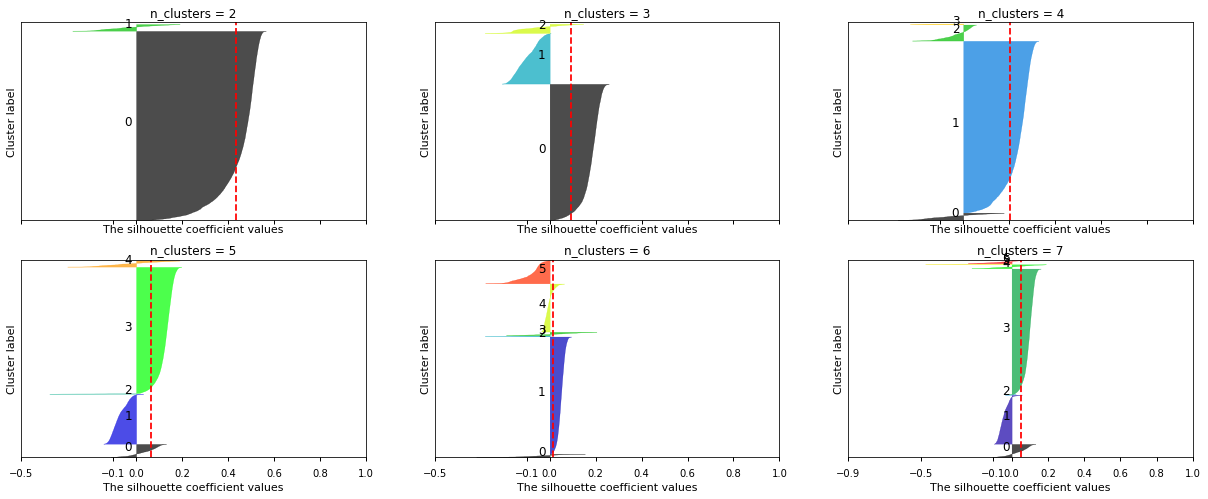
\includegraphics[width=1\linewidth]{clust_pca}
    \end{center}
    \caption{Silhouette analysis with a PCA (on top of preprocessing) retaining 95\% (yielding 165 components)}
    \label{clust_pca}
\end{figure}

We also tried wider ranges of clustering without much success, the scores still indicating that our clustering wasn't successful. Also what surprised us was that running multiple times the same algorithm on the same data would yield very variable results and therefore decreased our confidence in such model. 

We therefore tried to use additional tricks to improve our score and hopefully at the same time obtain more stable models. 

\subsection{Improving Scores}
As an extra performance metric, we decided to look at binary clustering as a prediction. That is, we would predict a cluster based on the majority class of labels in it. That would help us get metrics that we are more familiar with such as precision or recall but again this must be considered with extreme care as it doesn't translate the structure of the clustering (whether it is due to pure luck or not) and it relies on the existing labeling.

\subsubsection{Balancing the Dataset}
K-means is based on the assumption that clusters are of similar sizes, therefore we tried to balance the classes. This technique could seem incompatible with our aim to correct the labels. Indeed, by balancing we may discard false negatives from the 'healthy' class. But if we manage to find a correct clustering we could later use the cluster centers in order to cluster all the points using their distance to each center. 

Different techniques of data balancing exist but given our choice at the database level to subsample the sick class we remained in the same strategy at the data analysis level. 


\begin{figure}[ht]
    \begin{center}
    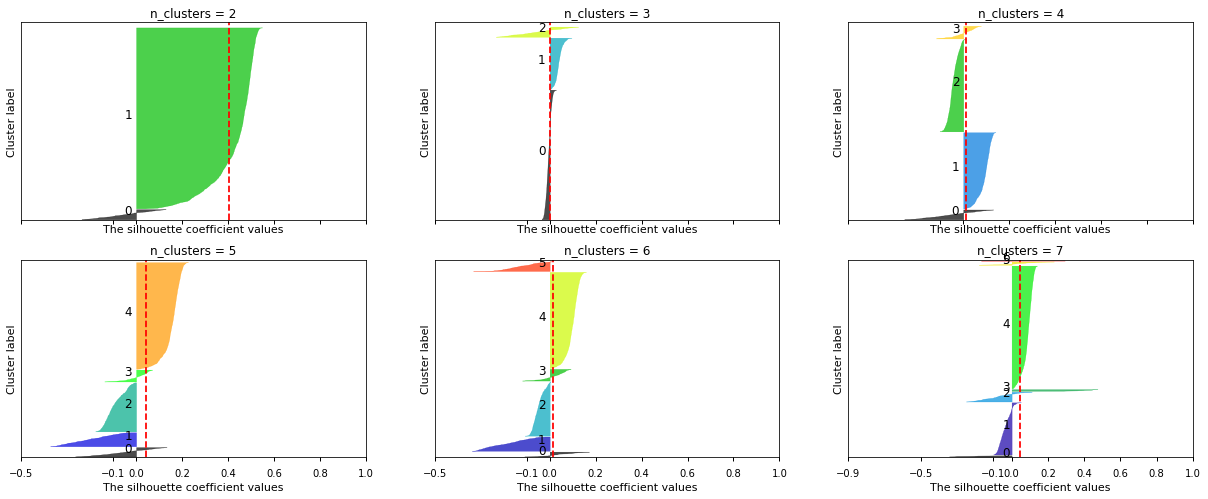
\includegraphics[width=1\linewidth]{clust_balanced}
    \end{center}
    \caption{Silhouette analysis with balanced class (on scaled and balanced data)}
    \label{clust_bal}
\end{figure}

One can observe on figure~\ref{clust_bal} that the scores are still fairly low. If we look closer at the binary clustering that is the most promising score of 0.4065, we obtain table~\ref{clust_clas}. It shows that either we are very wrong in the way we label data or there isn't a structure that can be exploited by K-Means.

\begin{table}[h]
\begin{center}
\begin{tabular}{c c c c c}
\hline
\textbf{Cluster interpretation} & \textbf{Desc} & \textbf{Counts} & \textbf{Label Proportion} & \textbf{Cluster proportion}\\ 
\hline\hline
\multirow{2}{*}{Healthy}  	& True negatives & 1140 & 97.94\% & 51.65\%\\
						  	& False negatives & 1067 & 91.68\% & 48.35\%\\
\hline
\multirow{2}{*}{Sick}  	& False positives & 24 & 2.06\% & 19.83\%\\
						  	& True positives & 97 & \textbf{8.33\%} & \textbf{80.17\%}\\
\end{tabular}
\end{center}
\caption{\label{clust_clas}Binary clustering interpreted as binary classification (balanced classes). On the sick class, we observe Recall$=8.33\%$ and Precision$=80.17\%$}
\end{table}

\subsubsection{Combining Dimensionality Reduction With Balanced Classes}
Because the score increased both thanks to class balancing and dimensionality reduction we combined both. We evaluated the average silhouette score for different levels of retained variance as shown in figure~\ref{clust_pca_diff_lev}. Even though we increased the average silhouette score of binary clustering we are still not obtaining scores that would allow us to present the clustering to the expert and check its output. 

\begin{figure}[ht]
    \begin{center}
    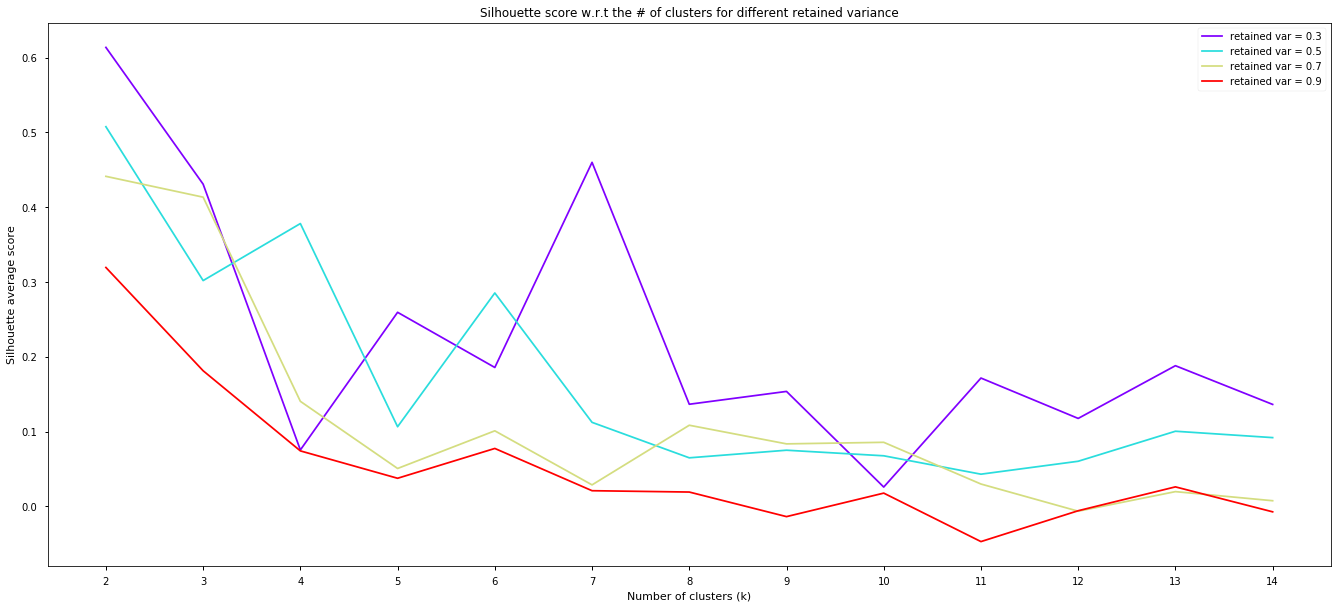
\includegraphics[width=1\linewidth]{clust_pca_diff_lev}
    \end{center}
    \caption{Average silhouette score for different levels of retained variance and different numbers of clusters (PCA+balanced classes)}
    \label{clust_pca_diff_lev}
\end{figure}

An attempt was also made at using LDA in combination of balanced classes with promising results on binary classification with $(R=50.515\%,P=81.667\%)$, unfortunately the average silhouette score of 0.1201 again revealed the poor structure that this clustering displayed and was hence abandoned. 

\vspace{1\baselineskip}
After this initial attempt at clustering, in concert with the business intelligence team we decided to move to classification. First of all, we couldn't display any clustering model that would be trustworthy. Also the lack of resources in the HFC support team made it complicated to check model outputs. 

To explain the difficulty experienced in our exploration of a correct clustering technique we thought of many reasons. The curse of dimensionality clearly plays a role in this as the notion of distance that is used both in the clustering algorithm and the scoring may be unusable. But also as a given problem may have different fixes, it would also be possible that 'symptoms' diverge with great magnitude preventing any clustering to reveal the underlying pattern. 

We focused back on classification as it usually relies on more complex models that can capture these differences in symptoms but also because the goal of the project is to provide a Proof-of-Concept to push the launch of a business project. Once such project goes live, the data can be sensibly enriched and cleaned to avoid the need for clustering as we will emphasise in section~\ref{sec:improving}. 

\section{Failure Prediction}
The predictions were the final goal of the project and our aim was to show that indeed we could predict the failures of some CPEs. As illustrated in previous steps, because the data could have been much improved and as models are only as good as the data they are fed, we focused on our top 'sick' predictions rather than focusing on the whole classification. This choice was again made after discussions with the supervisor of the project and the business intelligence team. It was made to reflect again the role of proof of concept of this project. 

We will present in this section first how we explored the different models that exist in this task by presenting the empirical research protocol both to find the best model but also to find the best way to assess the quality of a model. Then we will describe the fine-tuning of the model and give an overview on how each tuning step modified the performance metrics. Finally, we will discuss the model output by presenting some of the initial analysis that we conducted. 

\subsection{Model Exploration}
Model exploration is a trial and error exploration of binary classification that we suspect could help us predict CPE failures. We focused on 7 different such models combined with different preprocessing steps: Random Forests, Linear and Non-Linear Support vector machines, Gradient Boosting, k-Nearest Neighbors, Logistic Regression and Ridge Regression. This choice was arbitrary and there is a tradeoff in the number of models that can be evaluated and the fine-tuning of each model. 

In order to assess the quality of the model, we took care of cross validating our performance metrics. Cross validation aims at splitting the dataset into pairs of training and testing sets. It then successively, for each such pairs, trains the model and evaluate it on the test set. From the metrics series that we obtained, we can average them to obtain an unbiased estimate of the model on unlabelled data but also its variability thanks to the standard deviation of this series. 

\subsubsection{Initial research}
\paragraph{Performance Evaluation}
We need to compare the different models and in order to do such thing we would need a scoring technique of each model. We decided to use the recall and precision  as well as their average called F1-score (F1)~\cite{wiki:f1} on the 'sick' class on the top 20\% of predictions. 

But also we wished to use a graphical method to compare models. To achieve such goal we used Receiver Output Characteristic (ROC) curves~\cite{wiki:roc}. To put things simply, our model will output for each sample a probability that this sample belongs to the 'sick' class. To draw a ROC curve, we order such predictions by decreasing order of such probability, then starting from the bottom left, considering ordered prediction we go up if the prediction is correct and right if it isn't. Usually models are compared to the random classifier that is the diagonal joining bottom left to top right corners. This curve allows to focus on top predictions and see how well does the classifier performs on such.

To interpret this curve we privilege curves that are the steepest near the bottom left as it illustrates models that are very accurate on top predictions but also look at the overall area between the curve and the random classifier one. 

\paragraph{Standard Cross Validation (CV)}
The assumption that was formulated is that we could join all vectors in a single dataset without any consideration of their Day\textsubscript{0}. Then we built a 5-Fold~\cite{wiki:cv} on this pooled dataset.  

This allowed us to cross validate the three metrics (F1, P, R) and the ROC curves to have an unbiased estimator of the model on unseen data. 

Also we decided to balance the dataset before performing the split. This allowed us to ensure that splits would have homogeneous number of 'sick' representatives. 

\paragraph{Results}
For each model that we considered we explored both PCA and LDA given the good results yielded during the clustering attempt. For each combination of PCA and LDA we briefly explored different\footnote{Depending on the complexity of the model and therefore its training time, we could explore from 4 to 20 different values in ranges that we suspected as being the most appropriate.} model parameters to compare coarse tuned models. 

We report in table~\ref{initial_results} the performance of the coarse tuned model for each combination. We used the F1-Score on the top 20\% predictions as a single model score.

\begin{table}[h]
\begin{center}
\begin{tabular}{c c c c c c}
\hline
\textbf{F1(\%)} & \textbf{Model} & \textbf{Dim. Red.} & \textbf{Parameter} & \textbf{P(\%)} & \textbf{R(\%)}\\ 
\hline\hline
91.704730 & Random Forests & PCA & 5000 & 84.73 & 100\\
89.387325 & Non Linear SVM & PCA & 1 & 80.86 & 100\\
89.282233 & Gradient Boosting & PCA & 500 & 80.86 & 100\\
88.128110 & Gradient Boosting & LDA & 27 & 78.92 & 100\\
87.946957 & Logistic Regression & PCA & 1 & 78.49 & 100\\
87.864028 & Linear SVM & LDA & 0.01 & 78.49 & 100\\
86.868263 & Ridge Regression & LDA & 7.742637 & 76.99 & 100\\
86.868263 & Ridge Regression & LDA & 7.742637 & 76.99 & 100\\
\end{tabular}
\end{center}
\caption{\label{initial_results}Best results of the initial exploration order by decreasing F1-score on the top 20\% predictions.}
\end{table}

\textit{Nota Bene: the recall is the recall only computed by considering the top 20\% of predictions which could be confusing with later results. Here when $R=100\%$ it means that all the positives in the top 20\% predictions were identified as positives. This is undesirable but because of our wrong cross validation as we will explain it in the following paragraph we decided not to invest more work on this exploration but corrected it at a later time. We will discuss how our model selection strategy fails and how we corrected it in subsequent iterations.}

\begin{figure}[h]
\begin{center}$
\begin{array}{cccc}
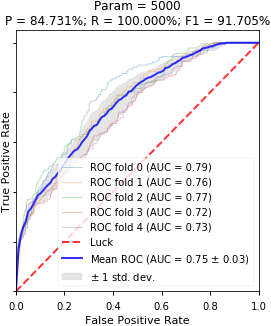
\includegraphics[width=1.4in]{ROC_RF} &
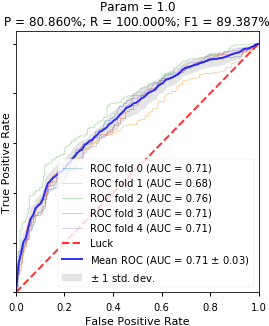
\includegraphics[width=1.4in]{ROC_NSVM} &
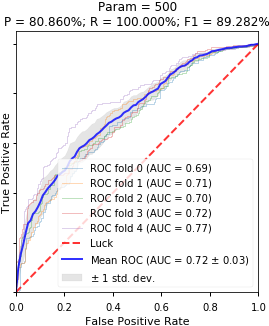
\includegraphics[width=1.4in]{ROC_GB} &
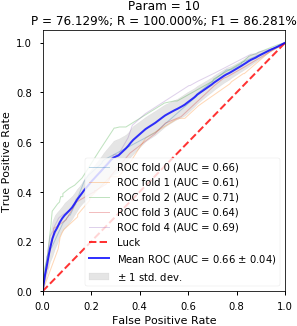
\includegraphics[width=1.53in]{ROC_GBLDA} 
\end{array}$
\end{center}
\caption{\label{ROC_init} ROC curves for the top four models (Left to right: Random Forests, Non-linear SVM and Gradient Boosting with PCA followed by Gradient Boosting with LDA)}
\end{figure}

\vspace{\baselineskip}
These results seem promising and Random Forests provide ideal performance on top predictions as we can also witness it on the ROC curve (c.f. Figure~\ref{ROC_init}) that is very steep and also presents the highest area under the curve. This means that even over all predictions, random forest outperforms the 3 other models. The model may require some extra tuning given its observable variability. 

\subsubsection{Improving Our Model Selection Process}
\paragraph{Problematic CV} Once we obtained such results we discovered that our estimate was incorrect. We tried to analyse how many days we could wait between training and predicting. In order to test this we needed to have a test set with dates that are non-overlapping with the training set. Even with 0 days past between the training and testing the classification metrics significantly dropped. The optimal model displayed above when tested on a test set made of 5 days yielded $P=51.25\%$. 

This proved the assumption that we formulated for the cross validation to be erroneous. It seems as if by training on same days as testing we overfit and overestimate performance metrics.	

\paragraph{Designing a New CV Strategy}
This pushed us to change the way we estimated the performance of our classifier. In order to have non-overlapping testing and training dates, we changed how we build each fold:
\begin{itemize}[noitemsep]
	\item From the full dataset, we derive the list of distinct dates and shuffle it. We end up with random indices $i$ for each date.
	\item To build a k-fold we assign day $i$ to the fold $i \text{ mod } k$ to homogeneously distribute dates over folds.
	\item Then we balance each training sets induced by each possible combination of $k-1$ folds.
\end{itemize}
With this strategy we ensure that we have balanced training sets as well as distinct dates between the training and testing sets. Figure~\ref{CV_comparison} illustrates the significant drop in estimated performance for the same model between the two CV techniques. 

\begin{figure}[h]
\begin{center}$
\begin{array}{cc}
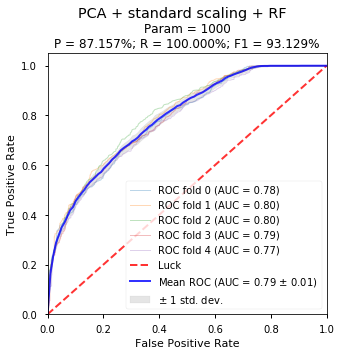
\includegraphics[width=2in]{old_cv} &
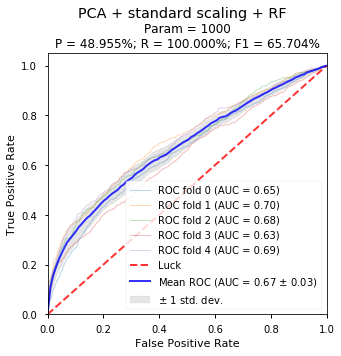
\includegraphics[width=2in]{new_cv} 
\end{array}$
\end{center}
\caption{\label{CV_comparison} Comparing old cross validation performance estimation (left) with the new one (right) on a Random Forest with 1000 trees with a PCA and standardised data}
\end{figure}


\paragraph{Graphical Performance Evaluation}
We would like to improve the previous model performance evaluation techniques and we followed multiple steps to do so.

So far we've been focusing on the top 20\% predictions in order to express the tradeoff between precision and recall on the 'sick' class. Nevertheless another technique would allow us to encapsulate such tradeoff. We could decide on different cutoff probabilities and look at the precision and recall for each. The cutoff probability is the value of the sick probability output by the model from which we start labeling samples as sick.

Also we let go of the ROC curve for Precision-Recall (PR) curves also called Calibration curves. These curves plot the precision against recall. Indeed it will be better in identifying good models in our imbalanced case (our test sets are left unbalanced). Suppose that we have a dataset with $500,000$ samples and only $100$ sick ones. and consider two algorithms:
\begin{itemize}[noitemsep,topsep=0pt]
	\item $\mathcal{A}_1$: 90 relevant out of the 100 identified
	\item $\mathcal{A}_2$: 90 relevant out of the 1000 identified
\end{itemize}
In our use case we would clearly prefer $\mathcal{A}_1$ over $\mathcal{A}_2$. Nevertheless if we compare PR and ROC curves we see that the first one distinguishes more easily the best algorithm:
\begin{itemize}
	\item ROC: 
		\begin{itemize}[noitemsep,topsep=0pt]
		\item $({TPR}_1,{FPR}_1)=(0.9,10/499,900)$
		\item $({TPR}_2,{FPR}_2)=(0.9,910/499,900)$
		\item Hence $|{FPR}_1-{FPR}_2|= 1.8\times 10^{-3}$
		\end{itemize}
	\item PR: 
		\begin{itemize}[noitemsep,topsep=0pt]
		\item $({P}_1,{R}_1)=(0.9,0.9)$
		\item $({P}_2,{R}_2)=(0.09,0.9)$
		\item Hence $|{P}_1-{P}_2|= 0.81$, wish shows that we distinguish models much more easily with such technique.
		\end{itemize}
\end{itemize}

We also had to derive a strategy to be able to cross validate a PR curve over different folds. Indeed, linear interpolation in the PR space yields an overly optimistic performance estimate~\cite{PRcurve} and because the probability thresholds used to build the curve for each fold may be different there isn't a trivial way to average curves. As suggested by past research~\cite{apples}, we will concatenate predictions and real targets of each test set and consider the PR curve constructed from these pooled predictions and true label datasets as our mean PR curve.

\paragraph{Metrics}
We also changed the metric that is monitored in order to determine the optimal model. As the business use of predictions entirely differs depending on the level of precision on the 'sick' class, we decided to use three precision levels $\{70\%,80\%,90\%\}$ that would be usable by business. We display on top of the PR curve the maximum recall that can be achieved for such precision. These metrics are computed on each fold and averaged overall. 

In order to determine the optimal model we will focus on the area under the PR curve. This will not exclusively evaluate the performance on top prediction but ensures that overall the model is optimal.

\subsubsection{Improved Research}
We performed the same kind of exploration but this time we also decided to try each model also without any dimensionality reduction algorithm (on standardised data). Indeed as we shall discuss it in the next subsection we realised that we may be losing information and hurting the performance of classifiers by blindly performing such compression.

\begin{table}[h]
\begin{center}
\begin{tabular}{c c c c c c c}
\hline
\textbf{Model} & \textbf{Dim. Red.} & \textbf{Parameter} & \textbf{AUC}& \textbf{R\textsubscript{70\%}(\%)} & \textbf{R\textsubscript{80\%}(\%)} & \textbf{R\textsubscript{90\%}(\%)} \\ 
\hline\hline
Gradient Boosting 	& - 		& 50 		& 0.528025 & 25.23 	& 18.51 & 10.48 \\
Random Forests 		& - 		& 5000		& 0.517642 & 24.06 	& 16.88 & 5.39\\
Non Linear SVM  	& - 		& 1	 		& 0.482226 & 18.55 	& 10.40 & 4.33\\
Linear SVM 			& PCA 	& 0.215443 	& 0.466997 & 17.57 	& 10.84 & 3.99\\
Logistic Regression & PCA 	& 0.003360 	& 0.472952 & 20.38 	& 11.68 & 3.91\\
Ridge Regression 	& PCA 	& 27.825594 	& 0.459569 & 18.93 	& 8.66 	& 3.15\\
\end{tabular}
\end{center}
\caption{\label{improved_results} Best results of the improved research ordered by decreasing R\textsubscript{90\%} (Maximum recall for 90\% precision)}
\end{table}

\begin{figure}[h]
\begin{center}$
\begin{array}{ccc}
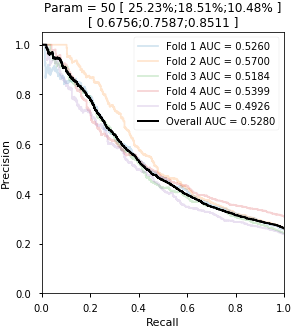
\includegraphics[width=1.8in]{PR_GB} &
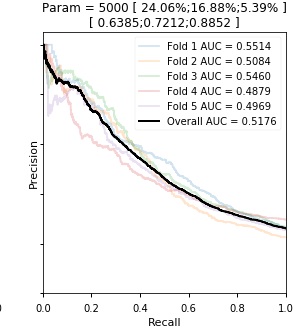
\includegraphics[width=1.8in]{PR_RF} &
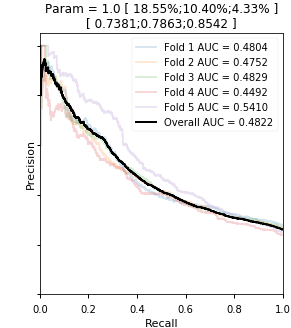
\includegraphics[width=1.8in]{PR_NSVM}
\end{array}$
\end{center}
\caption{\label{PR_curves} Precision Recall curves for the top 3 models obtained using the distinct date split. From left to right: Gradient Boosting, Random Forests, Non Linear SVM (always on standardised data). In the title of each graph we can observe the cutoff probability that yields the particular $(P,R)$ tuple.}
\end{figure}

We observe on Figure~\ref{PR_curves} that gradient boosting is more stable than the three other models as curves over different folds are grouped. The overall AUC is greater and we can see that the precision is high for more recall levels which also shows in R\textsubscript{90\%}, R\textsubscript{80\%} and R\textsubscript{70\%}. 

Given these results we focused on gradient boosting. The model is performing better without any dimensionality reduction as it requires fewer trees and is therefore simpler and quicker to train. 


\subsubsection{Understanding Classification}
\paragraph{No Dimensionality Reduction}
As advised by Felix Reisen from business intelligence, we wanted to check with the HFC support team if the most important features used by the model make sense. To perform such check we needed to look at the original features and not the components that are output by a dimensionality reduction technique. 

While trying out different ways to go from the most important components to the most important original features we tried to look at how the model performed without any dimensionality reduction. The overall better performance obtained pushed us to try to also explore this path in model coarse grain tuning and comparison. 

This strategy paid off as we can see that our top 3 models in previous subsection are not using any dimensionality reduction technique. 

\paragraph{Top 4 features}
Investigating the most important features of Gradient boosting gave us a good indication of the symptoms of failing CPEs. The most important feature was \texttt{OFFLINE\_PCT}, the percentage over Day\textsubscript{0} of offline hours. 


\begin{figure}[h]
\begin{center}$
\begin{array}{cc}
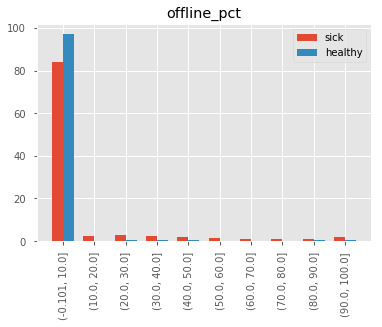
\includegraphics[width=2.55in]{most_imp_f_offline} &
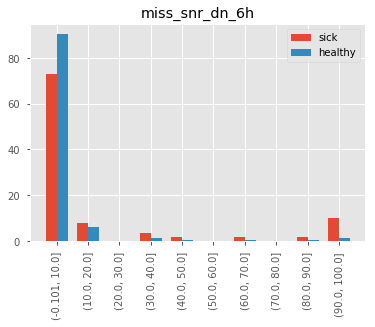
\includegraphics[width=2.5in]{most_imp_f_misssnr} \\
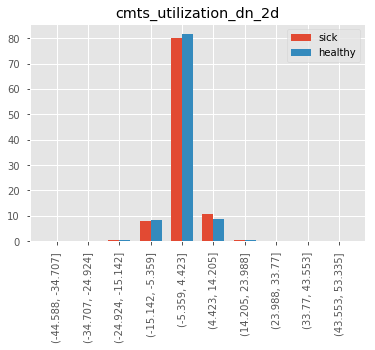
\includegraphics[width=2.5in]{most_imp_f_cmtsutil} &
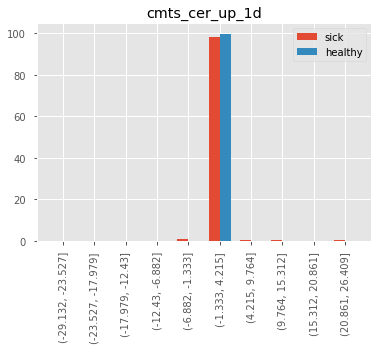
\includegraphics[width=2.5in]{most_imp_f_cmtscer}
\end{array}$
\end{center}
\caption{\label{most_important} 4 most important features distribution depending on the labels.}
\end{figure}


First of all, it is interesting as we also have a feature that gives the same percentage but over 6 hour windows but none are in the 4 most important features. That could indicate that customers do not have the same response time to call the technical help desk (THD) upon failure and therefore the percentage over 24 hours is more discriminative between classes. But also it gives us strong reasons to believe that a failing CPE is often time offline and this will influence the way me might handle predictions knowing that we may not be able to remotely service it. 

Also figure~\ref{most_important} confirms the usefulness of the CMTS level measurements as two such measurements are the 3rd and 4th most important features. The difference in distribution between labels couldn't be qualified as large, nevertheless we observe that for the \texttt{OFFLINE\_PCT} and \texttt{MISS\_SNR\_DN\_6H}, sick CPEs are less likely to be near zero.

According to Jonas, these indicators do make sense to identify internet problems and he expressed his desire to look at some CPEs predicted as failing to have more tangible results. We moved forward in our model tuning to be able to provide such examples. 

\subsection{Tuning Gradient Boosting}
Before we could present predictions to Jonas we had to fine-tune the model to make it optimal. We will present in this subsection how we fine-tuned the gradient boosting model, especially the new metric we decided to use, and the protocol we followed. Then we should look at the final model and visualise improvements added by the model relative to a baseline logistic regression.

\subsubsection{Protocol}
One should again consider that the proof of concept will not be used as a final model. Therefore an exhaustive grid search on each single parameters of the model may not be necessary. While we do want to display a well-adapted model, we are not interested in gaining 10\textsuperscript{th} of precision percentages as we only wish to prove that we can use the underlying patterns among failing CPEs to build a predictive model.

Also given the reduced time we had to tune the model and the diversity of hyper-parameters that can be adjusted, we had to limit the ones we would tune. Following popular practices~\cite{tuningGB}, we considered two steps:
\begin{itemize}
\item Tuning boosting parameters: focus on the number of estimators and the learning rate
\item Tuning tree based parameters: focus on the maximum depth of estimators and the minimum number of samples required to split a leaf node.
\end{itemize}
We are convinced that there is much greater work to be done on the data\footnote{As we should discuss it in chapter~\ref{chap:discussion}.} rather than the model itself, which is why we didn't spend too much time tuning the model. 

In order to report the performance of the model on the most recently collected dataset we present here the results based on a sample collected on the 27\textsuperscript{th} of June, time at which this section was draughted.

\subsubsection{Visualization}
At the time of this writing we realised that we forgot to test the model on unscaled data. Indeed due to its tree-based architecture, gradient boosting doesn't require scaling. Therefore we added the effect of this modification on our results but didn't use it in the model discussion as these tasks have been performed at an earlier time. 

\begin{table}[h]
\begin{center}
\begin{tabular}{c c c c }
\hline
\textbf{Model} & \textbf{R\textsubscript{70\%}} & \textbf{R\textsubscript{80\%}}& \textbf{R\textsubscript{90\%}}\\ 
\hline\hline
Linear Regression (scaled) & 24.8028\% & 15.6742\% & 4.7516\%  \\
Gradient Boosting (scaled) & 32.9851\% & 25.6919\% & \textbf{13.4116\%} \\
Gradient Boosting  &  \textbf{33.3239\%} & \textbf{26.2394\%} & 12.8978\%
\end{tabular}
\end{center}
\caption{\label{rec_models}Comparison of the performance (Maximum recall for a given precision) between our final model and the baseline.}
\end{table}

\begin{figure}[ht]
    \begin{center}
    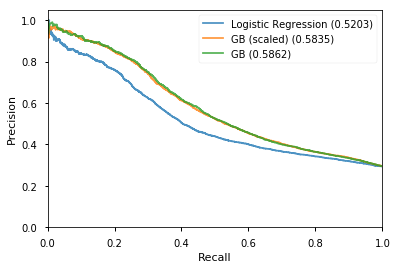
\includegraphics[width=0.6\linewidth]{images/model_comparison}
    \end{center}
	\caption{Calibration curves for final models against baseline}
    \label{model_comparison}
\end{figure}

On figure~\ref{model_comparison} we can observe that gradient boosting on unscaled data seems to be more stable at higher accuracy levels as the curve seems to be monotonous compared to the scaled version. This also illustrates the advantages of using PR curves to visually compare models: indeed if we were to look only at R\textsubscript{90\%} in table~\ref{rec_models}, we could believe the scaled version to perform better. We would like to note that we haven't displayed on the plot for visibility concerns the PR curve of each fold which means that one should be careful when comparing curves that could in reality describe variable models. 

\subsection{Model Discussion}
Once we had our final model, we were ready to analyse predictions. We first started by trying to predict a given day and go the same day to the HFC support team to review these predictions and see how they assess the quality of the model. Then we tried to perform again an analysis of how the number of days between training and predicting would affect the performance of the model. Finally, we briefly looked at one of our hypotheses regarding why standard cross validation caused a performance overestimation.

\subsubsection{Model Output Check}
On the 11\textsuperscript{th} of June, we trained the model on the dataset that we had collected up to this point and predicted potential failures. Once the model is tuned, we obtain 3 thresholds which are the probability thresholds that should help us reach particular $(P,R)$ pairs. 

At first we tried to use the highest threshold and found no MAC with a sick probability satisfying this threshold. Therefore we used the second threshold and one MAC was predicted as failing at this particular 'confidence level'. To leverage as much as possible the time that the HFC support team allocated to review our predictions with us we decided to also predict on all days that were not in the training set\footnote{It is important to remember that the training  set can only be constructed up to 8 days prior to the current date as explained in section~\ref{subsec:collecting}.}. That allowed us to generate more predictions and therefore come to the meeting with more material to analyse.

\begin{table}[h]
\begin{center}
\begin{tabular}{c c c p{90mm}}
\hline
\textbf{MAC} & \textbf{$p_\text{sick}$} & \textbf{Day\textsubscript{1}} & \textbf{Comment} \\ 
\hline\hline
\texttt{54:67:51:F4:0E:59} & 0.778949 & 10/06 & One HFC interface is continuously resetting, during this period the customer has no connection. Probably a hardware modem issue. \textbf{True positive}\\
\hline
\texttt{AC:22:05:9A:C2:21} & 0.892083 & 09/06 & Went offline for an extended amount of time. Nevertheless the many missing values could indicate a data polling issue. \textbf{False positive} but presents irregularities\\
\hline
\texttt{C4:27:95:17:77:A7} & 0.821313 & 07/06 & Lots of packets dropped on one of the channels, this can result for the customer in performance issues (service degradations). It is most probably a cabling problem that can be solved by the customer thanks to a replacement cable. \textbf{True positive}\\
\hline
\texttt{90:5C:44:BF:63:96} & 0.783860 & 06/06 &  We can see that levels were down for an extended period of time and went back up, which should indicate a technician intervention. We couldn't find it but given the similarities we can conclude that this is a \textbf{true positive}.\\
\end{tabular}
\end{center}
\caption{\label{checks} Four CPEs predicted as failing and review with the HFC support team}
\end{table}

As displayed in table~\ref{checks}, out of four predictions reviewed, three were true positives. Also Jonas expressed great satisfaction regarding the model as even the False positive presented some issues that could have thrown off the model. This reality check was necessary to ensure that the POC was pointing in the right direction as, up to this point, we based all our performance on metrics that rely on a ground truth that can be criticised. 

In order to review these predictions, the HFC team uses a tool based on SAA to display different health measurements of CPEs. In chapter~\ref{chap:discussion} we will discuss a specificity of this tool, as experts use value thresholds in order to track some performance indicators which could be leveraged by a future project.

\subsubsection{Time Gap Influence}
We repeated the analysis that we conducted earlier and made us realise our mistake using a standard cross validation. Because so far we can only train up to 8 days before the current date we looked at how the time between training and predicting influenced performances.

In order to estimate properly performances, we used all our available dates to cross validate our curves. We created multiple training set and testing set pairs with the correct time gap between them to generate our metrics. 

\begin{figure}[ht]
    \begin{center}
    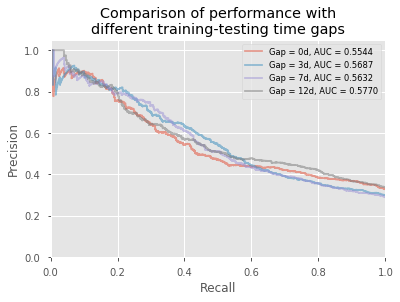
\includegraphics[scale=0.7]{time_gap}
    \end{center}
    \caption{Influence of time between the model is trained and used to generate prediction}
    \label{time_gap}
\end{figure}

Figure~\ref{time_gap} shows that we cannot identify a significant influence of time. Should there be an influence we would have expected to see the decreasing performance as time past. This supports the fact that the model can be used during an extended period of time without the need to be retrained every single day. 

\subsubsection{Same Weekday Training/Testing}
As stated earlier, our intuition regarding why our initial cross validation failed miserably was that training on dates that are also in the testing set may result in overfitting. We wondered whether we were not overfitting particular weekdays. To answer this question we created from the dataset, 7 subsets made only of identical weekdays. Then we generated our cross validated PR curves on each dataset to see if we would observe an increase of performance. By nature, this should not be conclusive as gradient boosted trees can use the \texttt{WEEK\_DAY} feature that we created to create sub-models for each day. 

\begin{figure}[h]
\begin{center}$
\begin{array}{c}
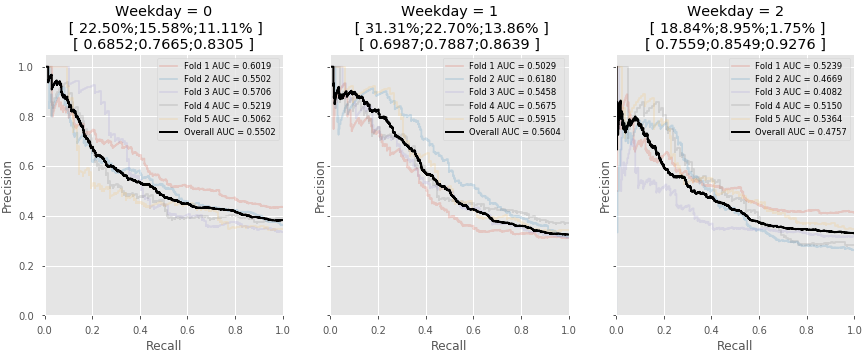
\includegraphics[scale=0.4]{weekdays_1} \\
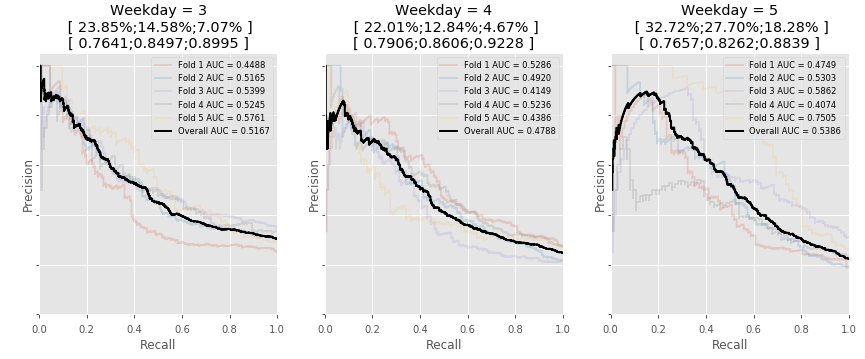
\includegraphics[scale=0.4]{weekdays_2} \\
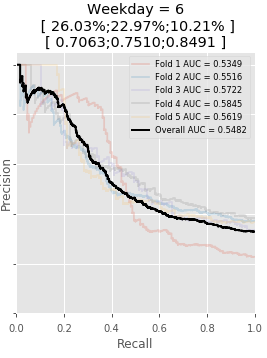
\includegraphics[scale=0.4]{weekdays_3} 
\end{array}$
\end{center}
\caption{\label{weekdays} Cross validated calibration curves for weekday subsets}
\end{figure}

Indeed, we can observe that the resulting performances (cf. figure~\ref{weekdays}) are not increased therefore ruling out our intuition that particular weekdays are overfitted. An interesting observation is the relative instability of the models on weekend days, compared to other days, that could confirm our intuition regarding the potential benefit of discarding weekend days from our analysis (cf. section~\ref{subsec:influence}). 

\vspace{\baselineskip}
We have successfully built a proof of concept that shows evidence of pattern in CPE failures that could be leveraged by UPC. Our intermediary analysis allowed us to have a better understanding of the data and also to spot some initial problems that would need to be mitigated in the future. Our attempt at clustering wasn’t conclusive but highlighted the power of some dimensionality reduction techniques and pushed for the need to have lower-dimensional space. Finally, the model exploration process presented iterative refinement of our goals and methods that will add great value to further research. 
\chapter{Discussion}
\label{chap:discussion}
Along previous lines we have identified points that need to be discussed regarding our choices and the way this proof of concept was engineered. This chapter will discuss these points to shed light on the pitfalls of our approach and potential points of improvements or further analysis that could drive the project forward. We won't extensively discuss each point but rather list some ideas.

\section{How Can We Use the Predictions?}
This question should have been solved prior to the project in order to set identifiable goals regarding the prediction algorithm. We collected some ideas regarding the potential way these predictions could be used.

When discussing with the team in charge of designing the support flows that are used by the THD agent, we discovered that most internet problems are solved without the real need for an agent (e.g. performing cabling checks, rebooting the CPE, ...). 

Also the call center is open from 8am to 10pm. We need to create the vectors for the past days in order to predict on the current day. Therefore the dataset can be generated from midnight to 1am. 

Some of the fix can be applied remotely. Nevertheless, as we noted previously, failing CPEs are more likely to be offline and therefore unreachable remotely. It is for this reason that we would propose the following steps:
\begin{enumerate}
	\item \textbf{Tentative remote fix}: upon detecting a failing CPE overnight, and for those that are reachable the company could try to apply the different remote fixes to the CPEs (e.g. reboot, update the firmware). Even if the prediction is wrong, during the night these fixes would go unnoticed by the customer. 
	\item \textbf{Self-Care}: then notify the customer that a potential problem has been identified with his/her CPE. Explain the remote steps that have been performed (if they have). Propose the same flow as the one used by the THD agent in a customer focused manner (vulgarised) to take him/her through the different steps that could solve the problem for example through a smartphone app. 
	\item \textbf{Shortcut}: only in the case where the customer couldn't fix his problem propose a reference that could be used to call the service center and save time to the expert by skipping all the checks that the customer performed on his own. In such case, the experts indicated that most probably the customer would need a swap or a truck roll.
\end{enumerate}

With such approach UPC could improve customer satisfaction by showing its pro-activity, but also it would save time to customers that wouldn't have to wait on the phone to perform basic checks. Finally, it would also reduce the workload put on the call center by restricting interaction with customers to the mere minimum and only in cases where it is necessary. 

\section{Improving Data}
\label{sec:improving}
A machine learning model is only as good as the data that it is fed. We have put together a quick business explanation of why we think that the data used by the model for now prevents business from leveraging entirely the value from their data management processes.

\subsection{Recall vs. Precision}
In order to check a prediction with an expert from the HFC support team, UPC would pay CHF8.54 for the workforce, while servicing a call costs CHF9 in terms of employee salary. These numbers estimated from employee salaries and average handling time show that a strategy of increasing the recall by dropping the precision would not be particularly successful. Indeed it costs approximately the same to service a call and to check a prediction which, moreover, won't fix the problem but simply identify it. 

\subsection{Building the Ground Truth Labelling}
We have highlighted on many occasions the limitations of using VIA as our only means to label vectors. First of all, we are discarding many cases out of the analysis for now. Out of the almost 3,000 calls received by UPC for technical help every day, this analysis considers approximately 112 CPEs every day as sick. On top of which the model can identify approximately 13\% at 90\% precision, 25\% at 80\% precision and 32\% at 70\% accuracy (cf table~\ref{model_comparison}).

A good start would be to change the way that data from the call center is collected to provide more reliable information. The MAC of the CPE that is being serviced isn't stored for now. It would be easy to collect it and would be a "quick win" to enrich the data. Also rather than using the FTR flag to decide whether the problem was fixed or not, customer feedback could be used. This would require the help of multiple stakeholders to adapt the servicing process but wouldn't require deep changes and therefore should be implemented without too much difficulty.

New sources of data could also be exploited. As any computer, a CPE collects software logs that identify potential problems. These logs could be leveraged in order to detect failing CPEs. We believe that these could be much more precise than using the correlation found between health measurements from the network and CPE failures. Moreover, these logs could be used to also diagnose CPEs with a deep sleep mode as we wouldn't need to access them every hour but could set up CPEs to transmit these logs every day at a given time (exiting deep sleep shortly for such purpose).

Also new sources of data could be leveraged and used to diagnose other flows of problems than internet ones. 

Finally, once predictions are being used, we could leverage customer feedback in order to enrich our labelling and correct potential mistakes. 

\vspace{\baselineskip}
The launch of an internal initiative around artificial intelligence could push different experts in the company to share their knowledge of UPC's assets. But also it would allow potential modification of internal processes to support the development of such solutions.


\section{Improving the Model}
This proof of concept was conducted in a limited time, with contained ressources and limited knowledge of the company's processes. This pushed for the development of a proof of concept rather than a production-ready project. We will discuss how this model could be modified and improved.

\subsection{Architecture}
Aggregation at the database level forced some choices to be locked in very early on. Indeed, raw data was being collected and aggregated daily which would mean that any modification of the dataset building process would force us to drop all data accumulated. 

Hopefully, UPC is now analysing the potential use of a big data infrastructure to provide more flexibility and computational power. Swiss regulations and corporate pressures prevent the company from using more scalable infrastructures as public cloud computing. This creates heavy upfront investments which explains the need for proof of concepts supporting such investments. A spark cluster for example would have allowed the data collection pipeline to be modified based on the performance of the classifier without the overhead of data collection time. 

\subsection{Data Representation}
With such architecture we would have been able to test for example different time windows to average measurements. The granularity that is necessary for the model could be cross validated but also the number of days of history for vectors. 

Moreover, many different representations could have been tried in combination with different preprocessing steps. 

\subsection{Leveraging Internal Knowledge}
The lack of resources dedicated by UPC to the project also prevented the model to be drastically improved. Indeed most of the project time was spent on exploring and understanding the different data sources owned by UPC. 

Knowledge is spread across different levels of the value chain and an official project could inspire some of these stakeholders to bring their own expertise to support the construction of an innovative tool. In terms of feature engineering, the knowledge of the different teams in charge of network maintenance but also the technical support and business intelligence could provide significant insights.

As an example, we discovered at a very late stage of the project that HFC support experts also had many thresholds that could be used to rule out 'flaps' of the signal but also to characterise alarming values of different health measurements (cf figure~\ref{thresholds}). This kind of knowledge could be combined with the model as a preprocessing step and prediction post processing in order to rule out some CPEs. 

\begin{figure}[ht]
    \begin{center}
    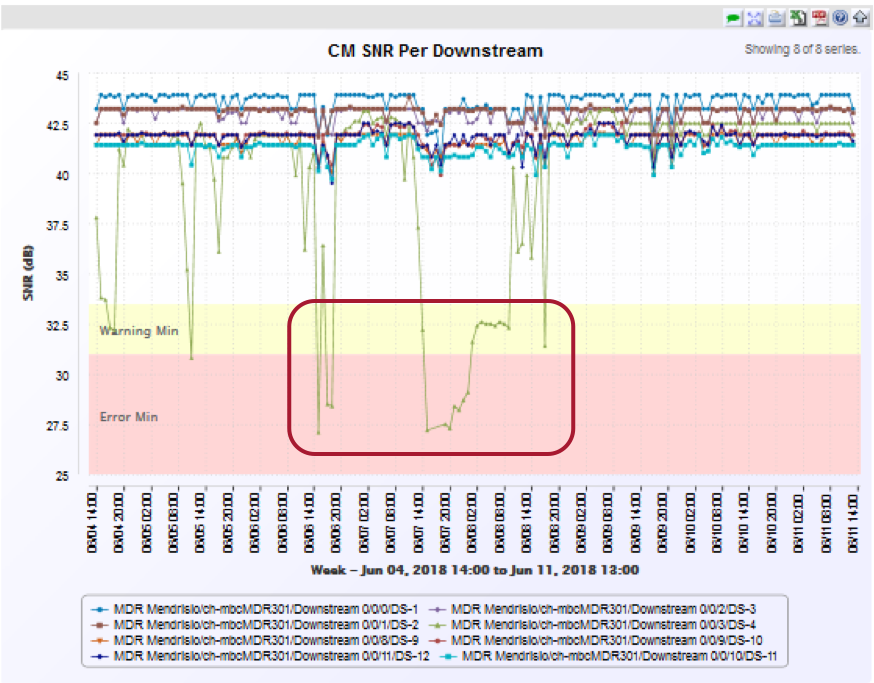
\includegraphics[width=1\linewidth]{thresholds}
    \end{center}
    \caption{Examples of graphs used by the HFC support team to diagnose problems. Here for the downstream sound to noise ratio (allowed us to detect a service degradation)}.
    \label{thresholds}
\end{figure}

\subsection{Complex Models}
Some more complex models could be combined with an improved dataset. The POC didn't contain any trial at deep learning given the engineering overhead as well as the results obtained with simpler model to support our goal.

\vspace{\baselineskip} 
Again, we could not emphasise enough the goal of this project that was to provide a proof of concept to the firm supporting the potential of the data it owns. This goal pushed many tradeoffs but the project can now be reused in order to shape a tool that could be put in production. 











\chapter{Conclusion}
This thesis thoroughly presents the empirical protocol that was followed in order to build a proof of concept in the scope of customer premises equipment failure detection.

We started by presenting the setup of the project and the technical background necessary to understand the work that has been done. This also allowed us to define the different resources available and derive the problem that was identified.

We moved to the description of the dataset construction. This phase certainly represented the most important of all. It consisted in gathering the different data sources available, selecting particular pieces of information that could prove to be useful for classification and finally determining how to best represent such information. The practical approach of data collection was also described as it required some engineering tricks to optimise our use of available resources.

Data analysis and machine learning was described in a trial and error spirit to justify our choices. The particular setup and goal of the project prevented us from using a classical pipeline. Clustering of the data to perform labelling propagation was attempted without much success but supported choices that could be later applied to the machine learning pipeline. 

Finally, we discussed our approach and tried to give recommendations regarding how we could use this proof of concept to take the project forward and implement it to increase the value to the customer and the company. 

To put things back in perspective, this \acrshort{poc} has drastically improved the set of tools that can be used by management to push for the development of internal competencies regarding Data Science. Out of the average of 0.2\% failing \acrshort{cpe}s, we have shown that we could detect 25\% of those with an 80\% accuracy proving the existence of an underlying pattern in the data that could be refined in order to proactively troubleshoot such failures. While this recall could seem low, it fits with the spirit of the project but also with the limited ressources that can be deployed to handle predictions at this stage. The project has sparked a lot of traction in the company both from the network and customer care business lines. 

Hopefully the desire of UPC to move to such analytical field will be confirmed in the future and leverage the research that has been conducted during this thesis to build an innovative solution.
\cleardoublepage
\appendix
\chapter{Repository}
All the work related to this project is available at the public repository: \url{https://github.com/hmoreau94/master-thesis}. The documentation of this repository is complete and won't be copied here. 


\chapter{Data Report}

\section{Continuous Variables - Frequency Plots}
\label{sec:continuous}
Figure~\ref{continuous-1} to~\ref{continuous-18} display the distribution of the different continuous features. 

\begin{figure}[ht]
    \begin{center}
    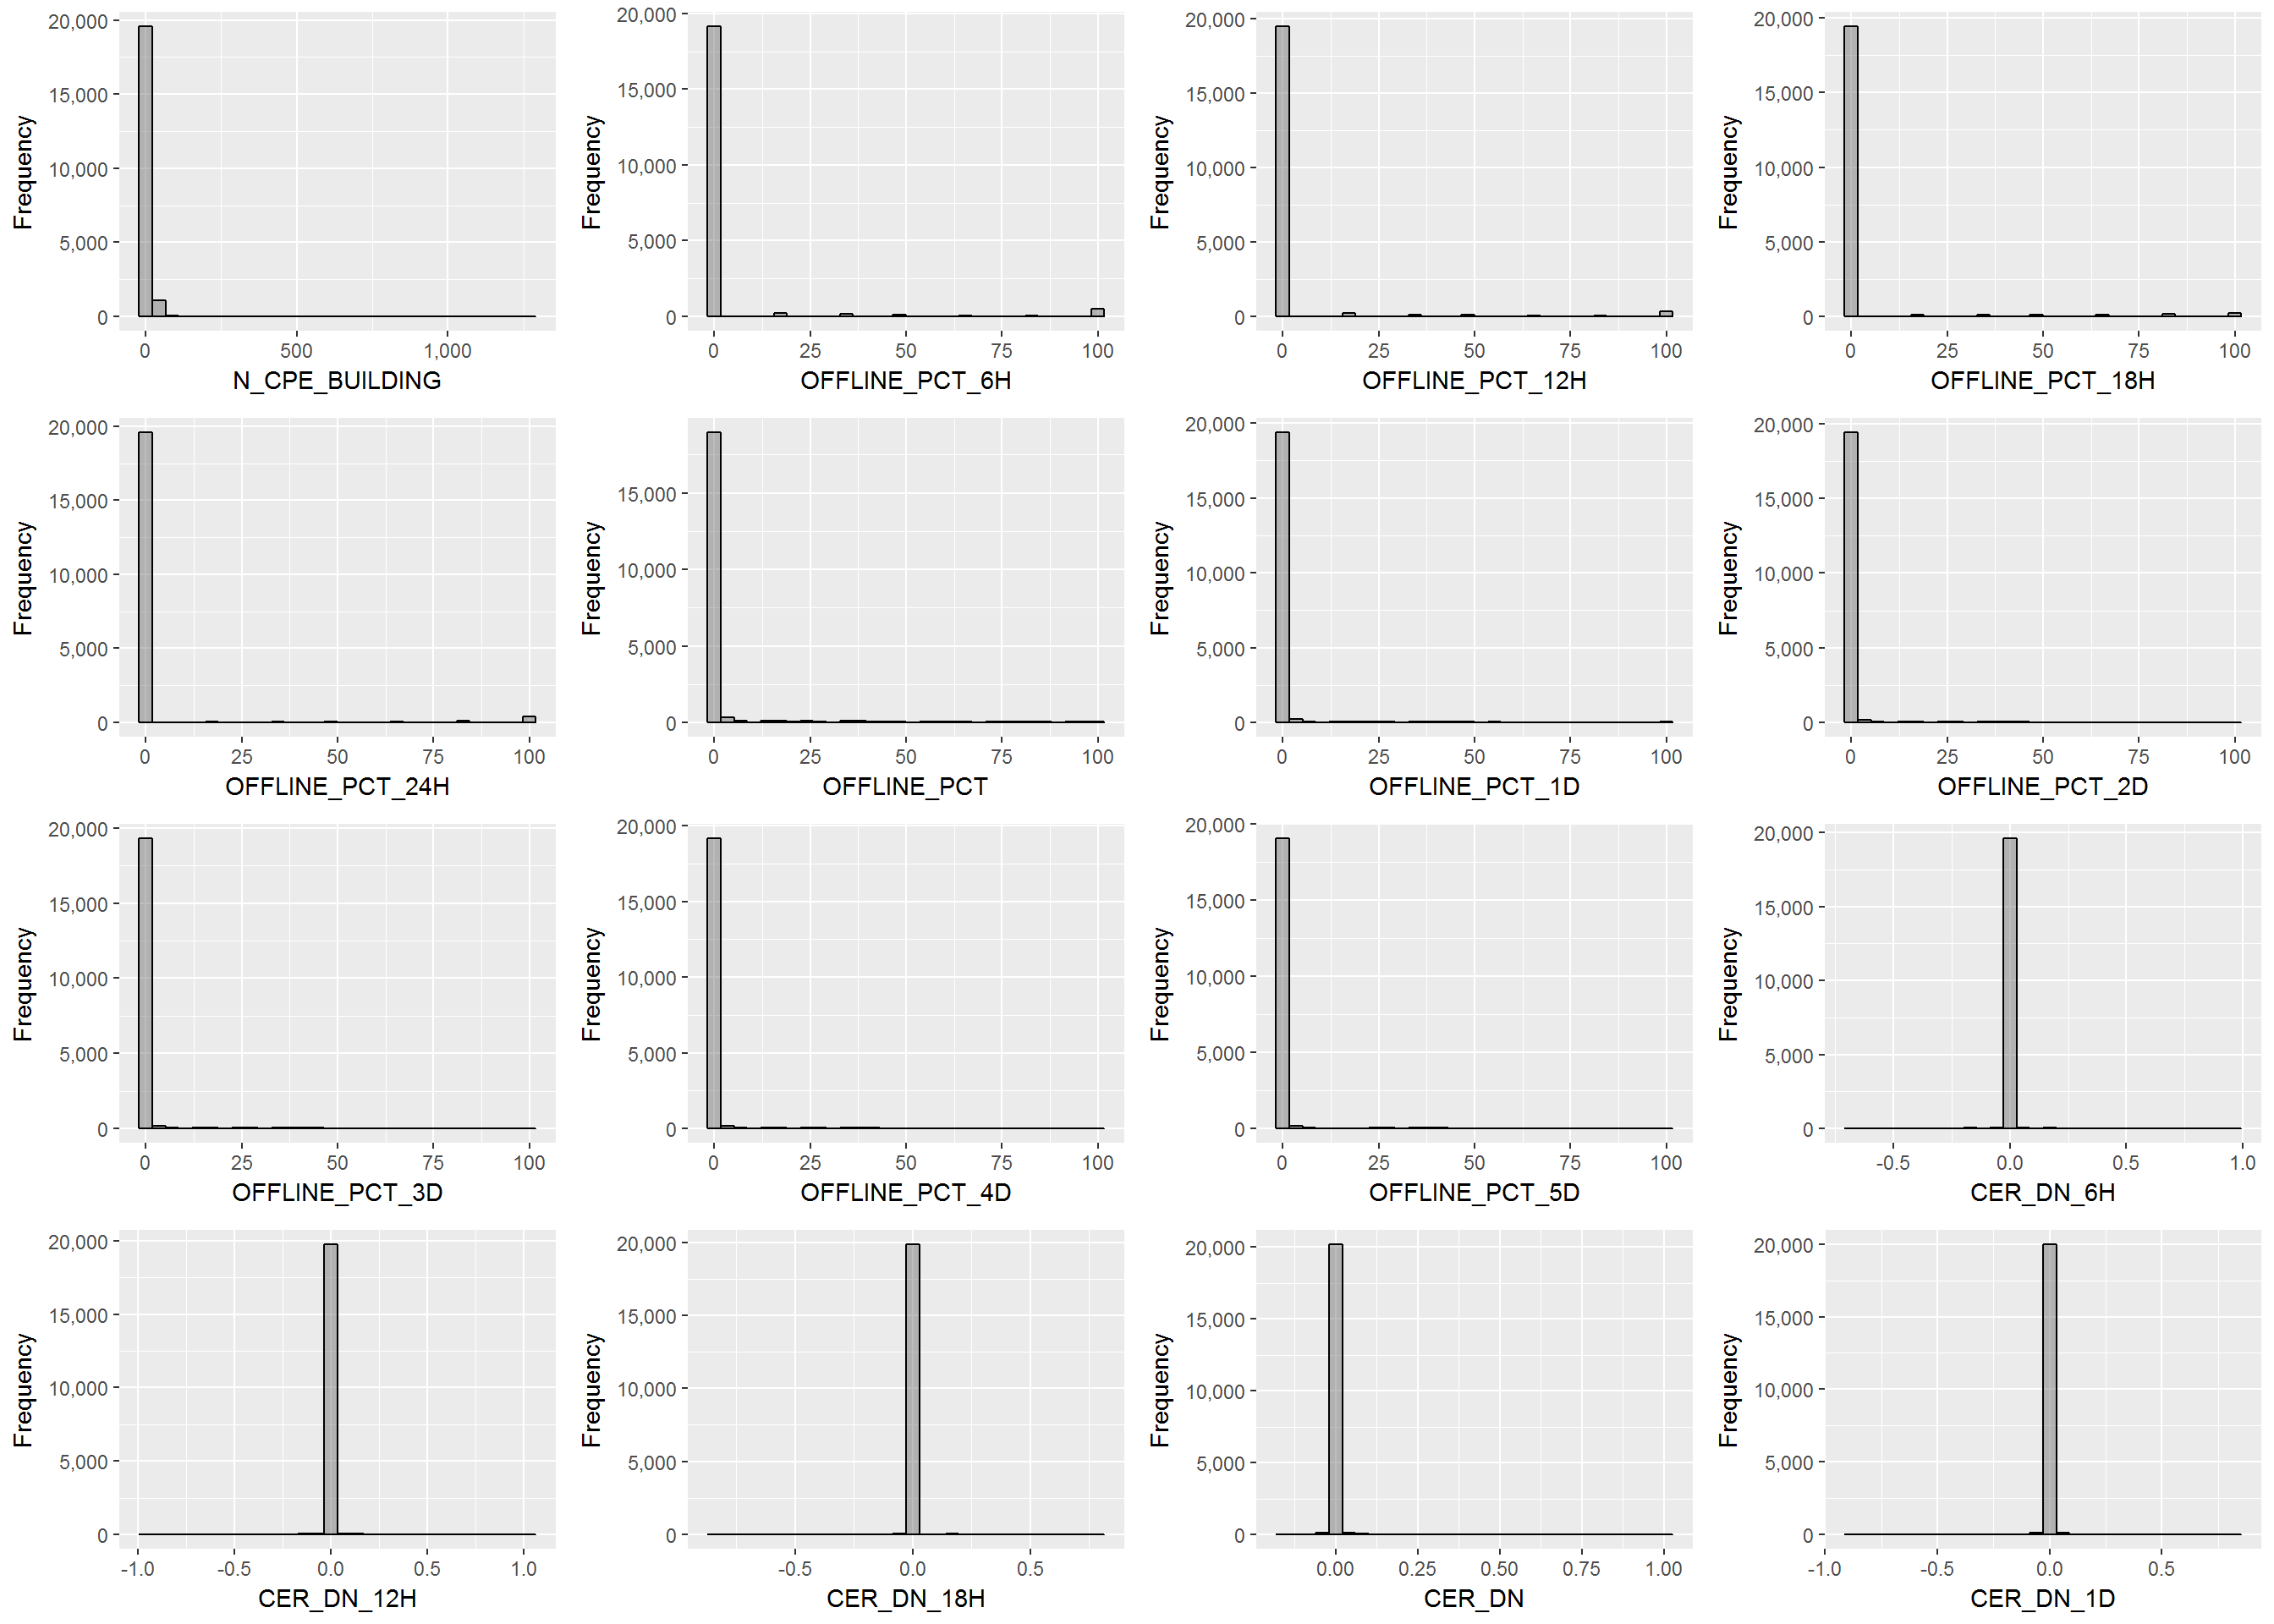
\includegraphics[width=1\linewidth]{continuous-1}
    \end{center}
    \caption{Part 1}
    \label{continuous-1}
\end{figure}

\begin{figure}[ht]
    \begin{center}
    \includegraphics[width=1\linewidth]{continuous-2}
    \end{center}
    \caption{Part 2}
    \label{continuous-2}
\end{figure}

\begin{figure}[ht]
    \begin{center}
    \includegraphics[width=1\linewidth]{continuous-3}
    \end{center}
    \caption{Part 3}
    \label{continuous-3}
\end{figure}

\begin{figure}[ht]
    \begin{center}
    \includegraphics[width=1\linewidth]{continuous-4}
    \end{center}
    \caption{Part 4}
    \label{continuous-4}
\end{figure}

\begin{figure}[ht]
    \begin{center}
    \includegraphics[width=1\linewidth]{continuous-5}
    \end{center}
    \caption{Part 5}
    \label{continuous-5}
\end{figure}

\begin{figure}[ht]
    \begin{center}
    \includegraphics[width=1\linewidth]{continuous-6}
    \end{center}
    \caption{Part 6}
    \label{continuous-6}
\end{figure}

\begin{figure}[ht]
    \begin{center}
    \includegraphics[width=1\linewidth]{continuous-7}
    \end{center}
    \caption{Part 7}
    \label{continuous-7}
\end{figure}

\begin{figure}[ht]
    \begin{center}
    \includegraphics[width=1\linewidth]{continuous-8}
    \end{center}
    \caption{Part 8}
    \label{continuous-8}
\end{figure}

\begin{figure}[ht]
    \begin{center}
    \includegraphics[width=1\linewidth]{continuous-9}
    \end{center}
    \caption{Part 9}
    \label{continuous-9}
\end{figure}

\begin{figure}[ht]
    \begin{center}
    \includegraphics[width=1\linewidth]{continuous-10}
    \end{center}
    \caption{Part 10}
    \label{continuous-10}
\end{figure}

\begin{figure}[ht]
    \begin{center}
    \includegraphics[width=1\linewidth]{continuous-11}
    \end{center}
    \caption{Part 11}
    \label{continuous-11}
\end{figure}

\begin{figure}[ht]
    \begin{center}
    \includegraphics[width=1\linewidth]{continuous-12}
    \end{center}
    \caption{Part 12}
    \label{continuous-12}
\end{figure}

\begin{figure}[ht]
    \begin{center}
    \includegraphics[width=1\linewidth]{continuous-13}
    \end{center}
    \caption{Part 13}
    \label{continuous-13}
\end{figure}

\begin{figure}[ht]
    \begin{center}
    \includegraphics[width=1\linewidth]{continuous-14}
    \end{center}
    \caption{Part 14}
    \label{continuous-14}
\end{figure}

\begin{figure}[ht]
    \begin{center}
    \includegraphics[width=1\linewidth]{continuous-15}
    \end{center}
    \caption{Part 15}
    \label{continuous-15}
\end{figure}

\begin{figure}[ht]
    \begin{center}
    \includegraphics[width=1\linewidth]{continuous-16}
    \end{center}
    \caption{Part 16}
    \label{continuous-16}
\end{figure}

\begin{figure}[ht]
    \begin{center}
    \includegraphics[width=1\linewidth]{continuous-17}
    \end{center}
    \caption{Part 17}
    \label{continuous-17}
\end{figure}

\begin{figure}[ht]
    \begin{center}
    \includegraphics[width=1\linewidth]{continuous-18}
    \end{center}
    \caption{Part 18}
    \label{continuous-18}
\end{figure}

\section{Categorical Variables - Frequency Plots}
\label{sec:categorical}
Figure~\ref{categorical} displays the distribution of categorical variables.
\begin{figure}[ht]
    \begin{center}
    \includegraphics[width=1\linewidth]{categorical-1}
    \end{center}
    \caption{Categorical variables}
    \label{categorical}
\end{figure}




\printbibliography

\end{document}

